\graphicspath{{chapt_dutch/}{intro/}{chapt2/}{chapt3/}{chapt4/}{chapt5/}{chapt6/}{chapt7/}}

% Header
\renewcommand\evenpagerightmark{{\scshape\small Chapter 5}}
\renewcommand\oddpageleftmark{{\scshape\small Consolidation and Research and Development approval}}

\hyphenation{}

\chapter[Longevity studies and Consolidation of the present \acs{CMS} \acs{RPC} subsystem]%
{Longevity studies and Consolidation of the present \acs{CMS} \acs{RPC} subsystem}
\label{chapt:5}

%****************************************** TESTING DETECTORS UNDER EXTREME CONDITIONS *****************************************************
\section{Testing detectors under extreme conditions}
\label{sec:extreme}
	
	The upgrade from LHC to HL-LHC will increase the peak luminosity from 10$^{34}$ \si{cm^{-2}.s^{-1}} to reach 5$\times$10$^{34}$ \si{cm^{-2}.s^{-1}}, increasing in the same way the total expected background to which the RPC system will be subjected to.
	Composed of low energy gammas and neutrons from $p$-$p$ collisions, low momentum primary and secondary muons, puch-through hadrons from calorimeters, and particles produced in the interaction of the beams with collimators, the background will mostly affect the regions of CMS that are the closest to the beam line, i.e. the RPC detectors located in the endcaps. {\color{blue} [To update.]}\\
	
    The 2016 data allowed to study the values of the background rate in all RPC system.
	In Figure~\ref{Fig:HL-LHC}, the distribution of the chamber background hit rate per unit area is shown at a luminosity of $5\times10^{34}cm^{-2}.s^{-1}$ linearly extrapolating from data collected in 2016 {\color{blue} [ref mentioning the linear dependency of rate vs lumi]}.
	The maximum rate per unit area at HL-LHC conditions is expected to be of the order of ${600}{Hz/cm^2}$ (including a safety factor 3).
	Nevertheless, Fluka simulations have conducted in order to understand the background at HL-LHC conditions.
	The comparison to the data has shown, in Figure~\ref{Fig:Fluka}, a discrepancy of a factor 2 even though the order of magnitude is consistent. {\color{blue} [Understand mismatch.]}\\
    
    \begin{figure}[!h]
		\begin{subfigure}{\linewidth}
		    \centering
			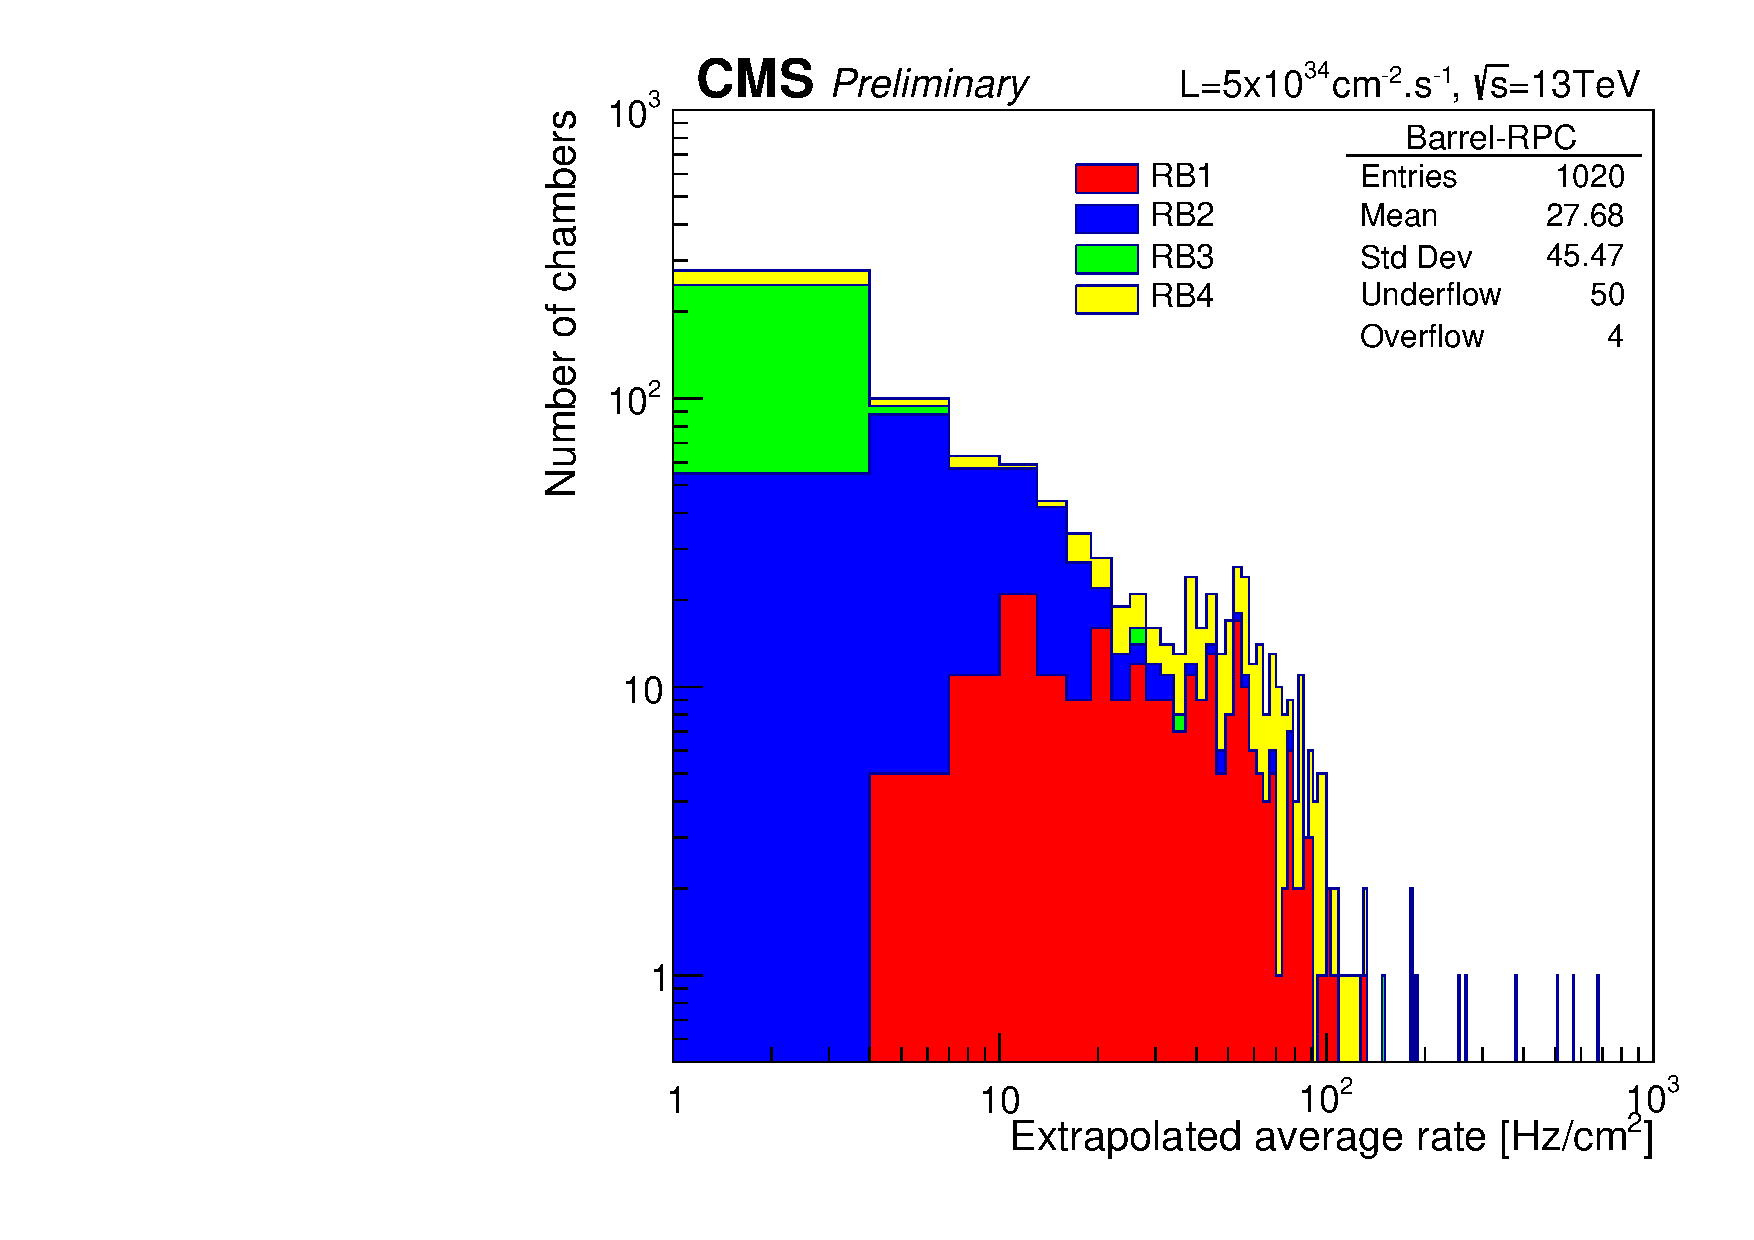
\includegraphics[width = \plotwidth]{fig/chapt5/Barrel-Roll-Rate-HL-LHC.pdf}\\
			\caption{\label{Fig:HL-LHC:Barrel}}
		\end{subfigure}
		\begin{subfigure}{\linewidth}
		    \centering
			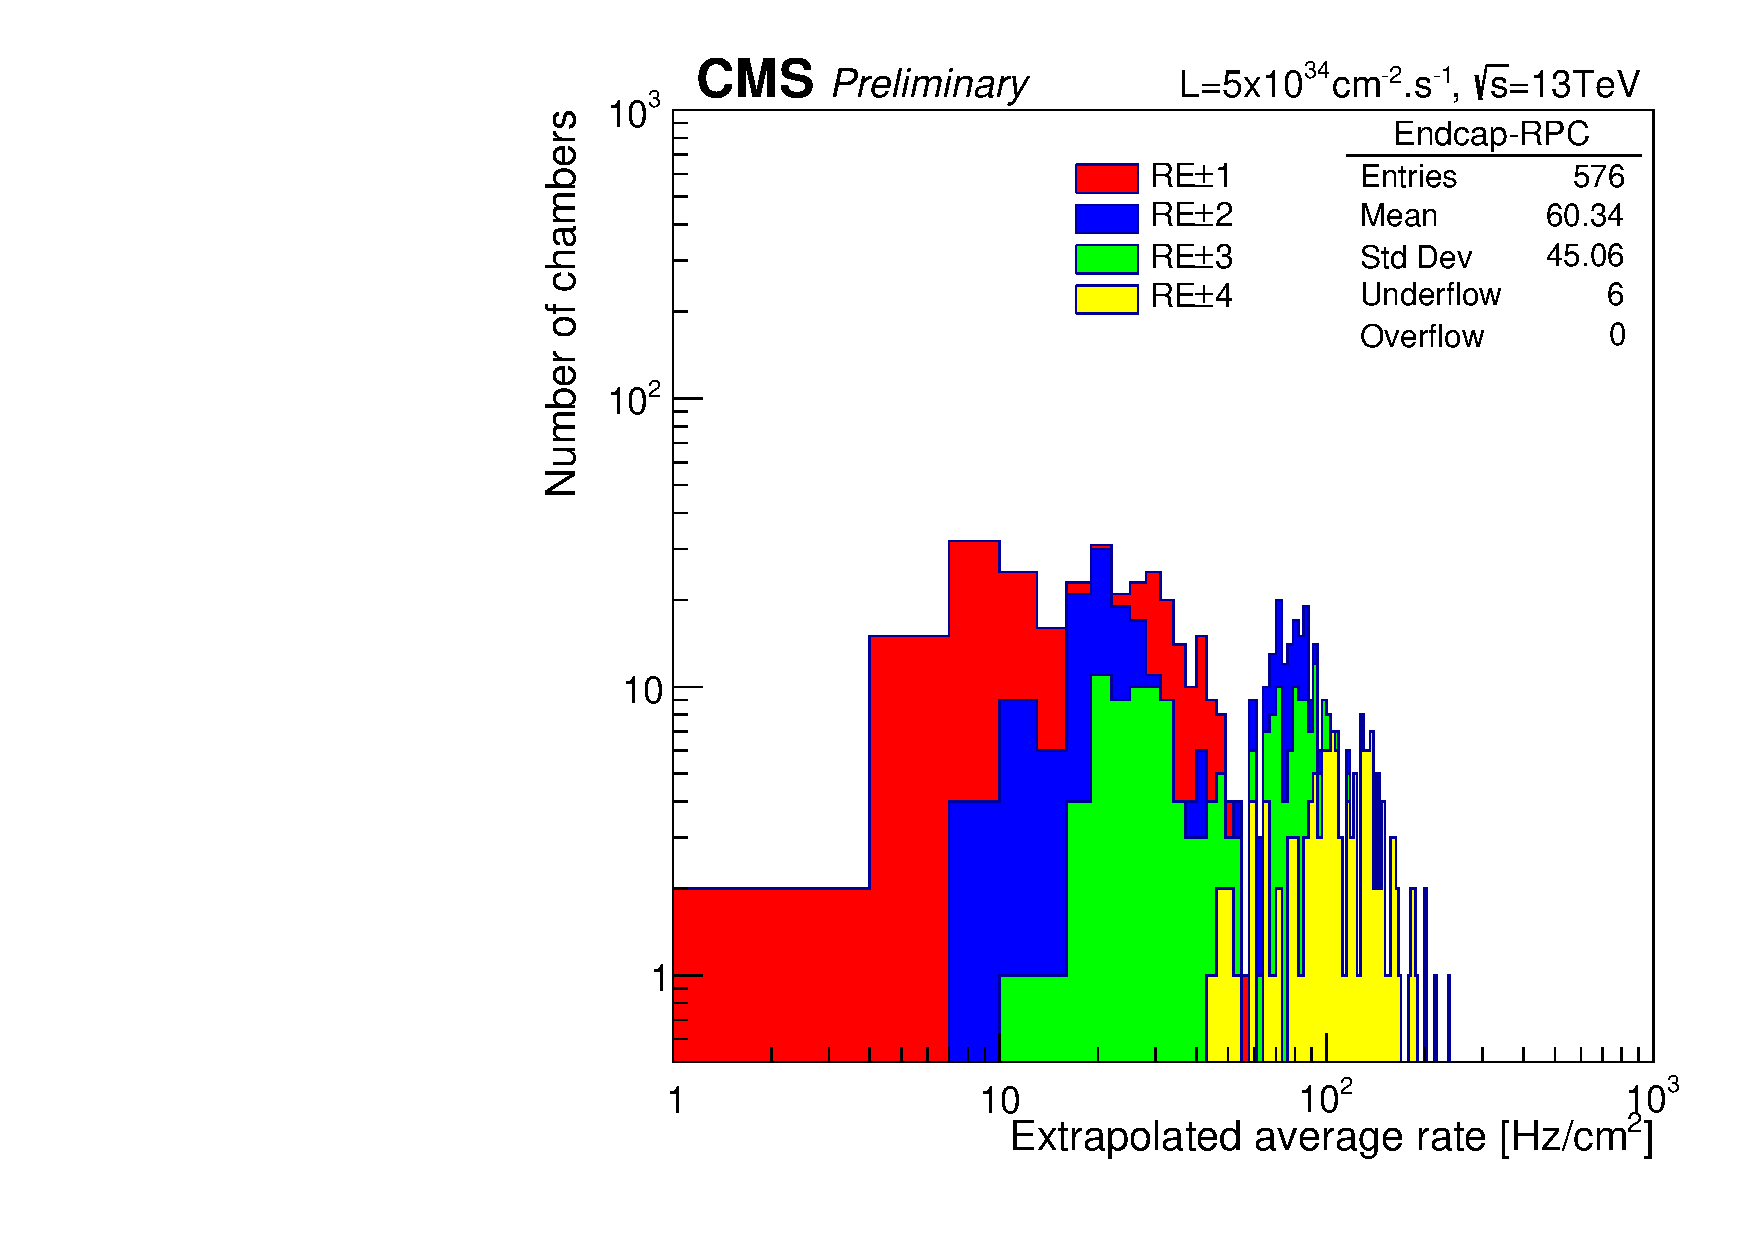
\includegraphics[width = \plotwidth]{fig/chapt5/Endcap-Disks-Rate-HL-LHC.pdf}
			\caption{\label{Fig:HL-LHC:Endcap}}
		\end{subfigure}
        \caption{\label{Fig:HL-LHC}(\ref{Fig:HL-LHC:Barrel}) Extrapolation from 2016 data of single hit rate per unit area in the barrel region. (\ref{Fig:HL-LHC:Endcap}) Extrapolation from 2016 data of single hit rate per unit area in the endcap region.}
    \end{figure}
    
    \begin{figure}[!h]
        \centering
        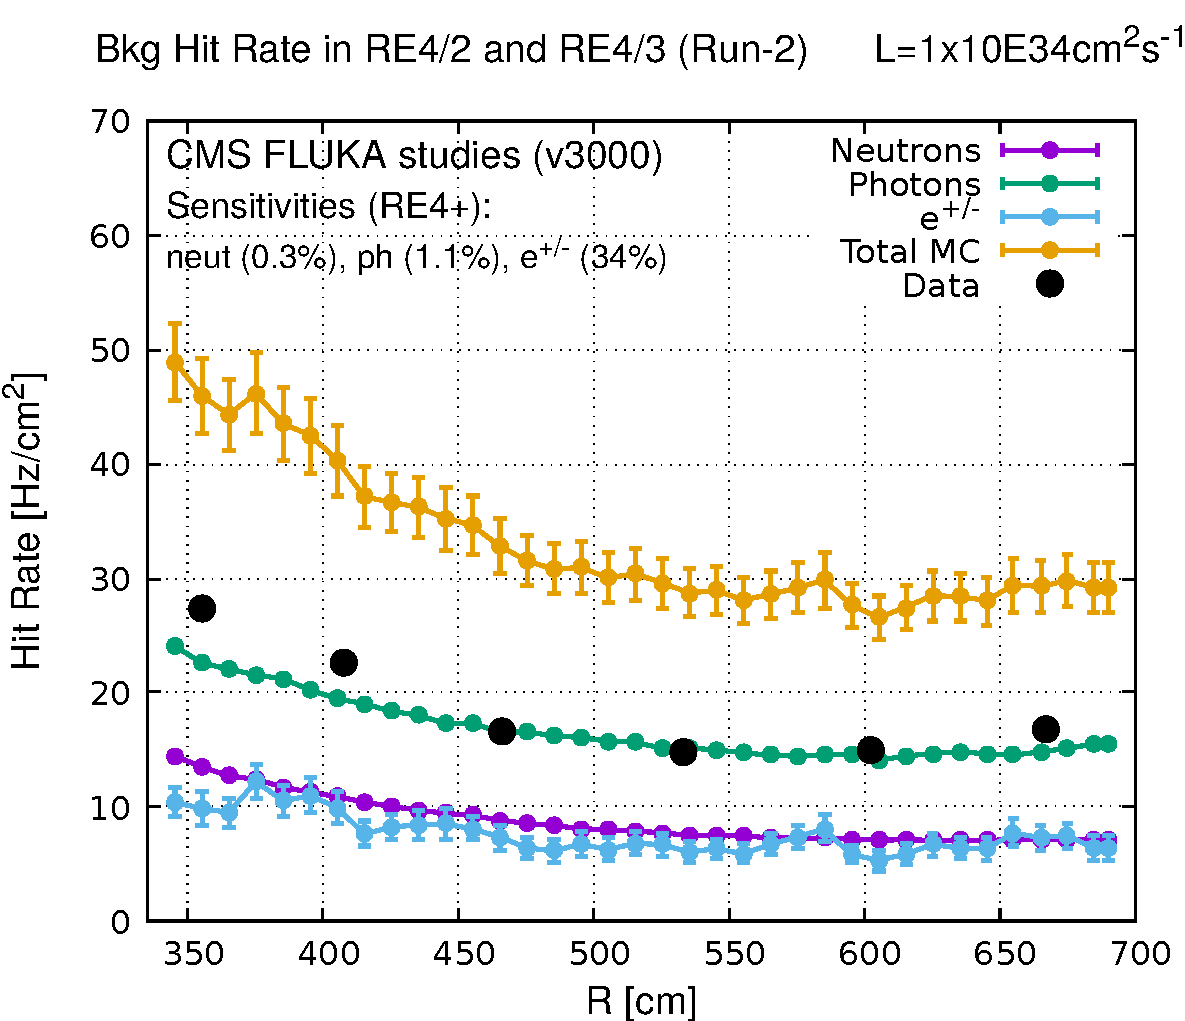
\includegraphics[width=\plotwidth]{fig/chapt5/RE4-Fluka.pdf}\\
        \caption{\label{Fig:Fluka} Background Fluka simulation compared to 2016 Data at $L=10^{34}cm^{-2}.s^{-1}$ in the fourth endcap disk region. A mismatch in between simulation and data can be observed. {\color{blue} [To be understood.]}}
    \end{figure}

	In the past, extensive long-term tests were carried out at several gamma and neutron facilities certifying the detector performance.
	Both full size and small prototype RPCs have been irradiated with photons up to an integrated charge of $\sim {0.05}{C/cm^2}$ and $\sim {0.4}{C/cm^2}$, respectively~\cite{GIF2004,AGING2009}.
	During Run-I, the RPC system provided stable operation and excellent performance and did not show any aging effects for integrated charge of the order of ${0.01}{C/cm^2}$.
    Projections on currents from 2016 Data, has allowed to determine that the total integrated charge, by the end of HL-LHC, would be of the order of ${1}{C/cm^2}$ (including a safety factor 3).
{\color{blue} [Corresponding figure needed.]}\\

	%****************************************** GAMMA IRRADIATION FACILITIES ********************************************************
	\subsection{The Gamma Irradiation Facilities}
	\label{ssec:Facilities}
		%****************************************** OLD GIF ******************************************************************
		\subsubsection{GIF}
		\label{sssec:GIF}
		
			Located in the SPS West Area at the downstream end of the X5 test beam, the \acf{GIF} was a test area in which particle detectors were exposed to a particle beam in presence of an adjustable gamma background~\cite{AGOSTEO1999}. Its goal was to reproduce background conditions these detectors would suffer in their operating environment at LHC. GIF layout is shown in Figure ~\ref{fig:GIFLayout}. Gamma photons are produced by a strong $^{137}$Cs source installed in the upstream part of the zone inside a lead container. The source container includes a collimator, designed to irradiate a \SIsurface{6}{6}{\meter} area at \SI{5}{\meter} maximum to the source. A thin lens-shaped lead filter helps providing with a uniform outcoming flux in a vertical plane, orthogonal to the beam direction. The principal collimator hole provides a pyramidal aperture of \SI{74}{\degree}$\times$ \SI{74}{\degree} solid angle and provides a photon flux in a pyramidal volume along the beam axis. The photon rate is controled by further lead filters allowing the maximum rate to be limited and to vary within a range of four orders of magnitude. Particle detectors under test are then placed within the pyramidal volume in front of the source, perpendicularly to the beam line in order to profit from the homogeneous photon flux. Adjusting the background flux of photons can then be done by using the filters and choosing the position of the detectors with respect to the source.\\
	
			\begin{figure}[!h]
				\centering
				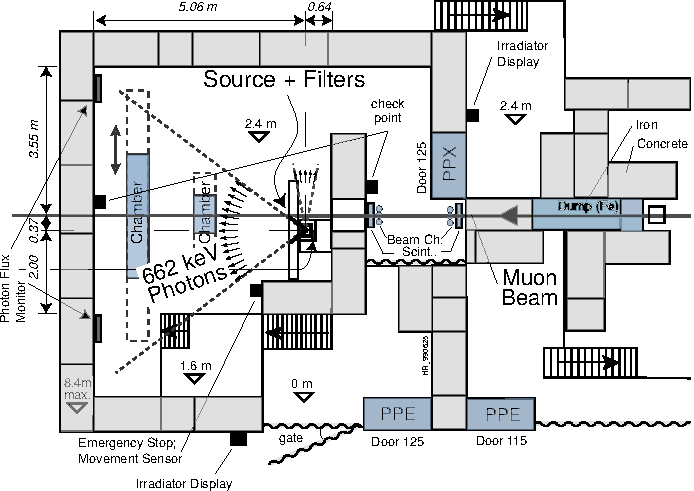
\includegraphics[width = \plotwidth]{fig/chapt5/GIF-Layout.pdf}\\
				\caption{\label{fig:GIFLayout} Layout of the test beam zone called X5c GIF at CERN. Photons from the radioactive source produce a sustained high rate of random hits over the whole area. The zone is surrounded by \SI{8}{\meter} high and \SI{80}{\cm} thick concrete walls. Access is possible through three entry points. Two access doors for personnel and one large gate for material. A crane allows installation of heavy equipment in the area.}
			\end{figure}
			
			As described on Figure~\ref{fig:CsSource}, the $^{137}$Cs source emits a \SI{662}{\keV} photon in 85\% of the decays. An activity of \SI{740}{\GBq} was measured on the 5$^{th}$ March 1997. To estimate the strength of the flux in 2014, it is necessary to consider the nuclear decay through time assiciated to the Cesium source whose half-life is well known ($t_{1/2}=$ \SIerror{30.05}{0.08}{y}). The GIF tests where done in between the $20^{th}$ and the $31^{st}$ of August 2014, i.e. at a time $t=$ \SIerror{17.47}{0.02}{y} resulting in an attenuation of the activity from \SI{740}{GBq} in 1997 to \SI{494}{GBq} in 2014.\\

			\begin{figure}[!h]
				\centering
				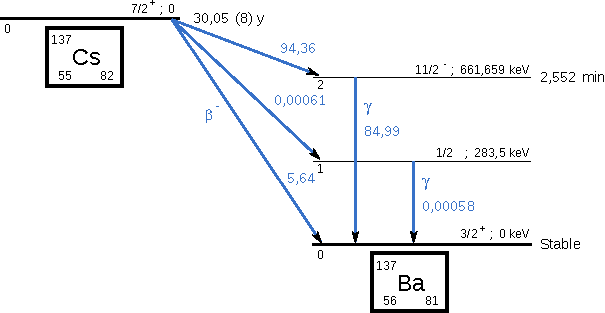
\includegraphics[width = \plotwidth]{fig/chapt5/Cs137.pdf}\\
				\caption{\label{fig:CsSource} $^{137}$Cs decays by $\beta^-$ emission to the ground state of $^{137}$Ba (BR = 5.64\%) and via the \SI{662}{\keV} isomeric level of $^{137}$Ba (BR = 94.36\%) whose half-life is 2.55 min.}
			\end{figure}
			
		
		%****************************************** NEW GIF ******************************************************************
		\subsubsection{GIF++}
		\label{sssec:GIF++}
		
			The \acf{GIF++}, located in the SPS North Area at the downstream end of the H4 test beam, has replaced its predecessor during LS1 and has been operational since spring 2015~\cite{JAKEL2014}. Like GIF, GIF++ features a $^{137}$Cs source of \SI{662}{\keV} gamma photons, their fluence being controlled with a set of filters of various attenuation factors. The source provides two separated large irradiation areas for testing several full-size muon detectors with continuous homogeneous irradiation, as presented in Figure~\ref{fig:GIFpp-Layout}.\\
			
			\begin{figure}[!h]
				\centering
				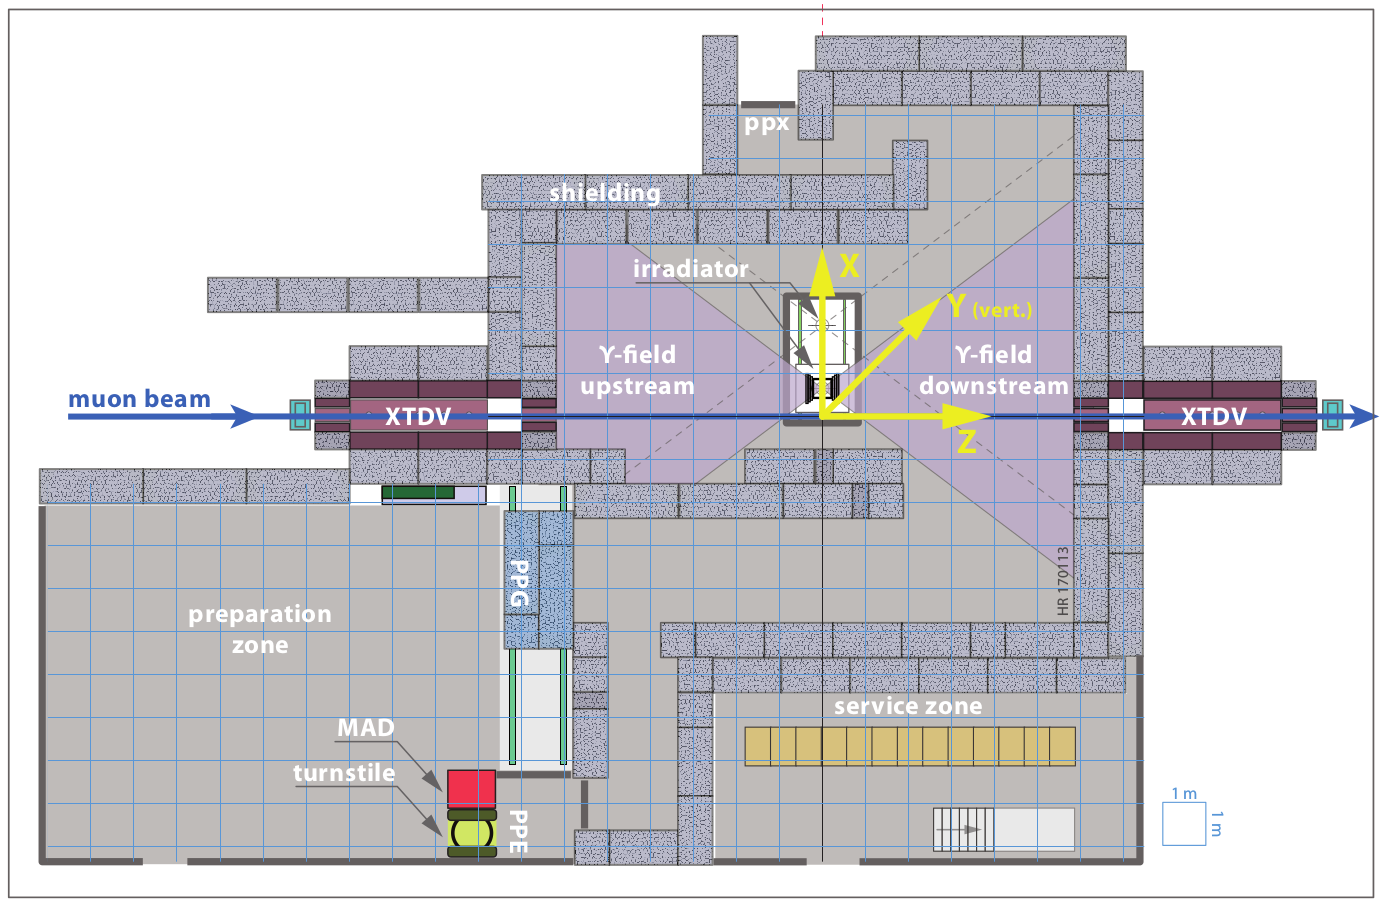
\includegraphics[width = \plotwidth]{fig/chapt5/GIFpp-Layout.png}\\
				\caption{\label{fig:GIFpp-Layout} Floor plan of the GIF++ facility. When the facility downstream of the GIF++ takes electron beam, a beam pipe is installed along the beam line (z-axis). The irradiator can be displaced laterally (its center moves from $x=$\SI{0.65}{m} to \SI{2.15}{m}), to increase the distance to the beam pipe.}
			\end{figure}
			
			 The source activity was measured to be about \SI{13.5}{TBq} in March 2016. The photon flux being far greater than HL-LHC expectations, GIF++ provides an excellent facility for accelerated aging tests of muon detectors.\\
			 
			\begin{figure}[!h]
				\begin{subfigure}{\linewidth}
				    \centering
					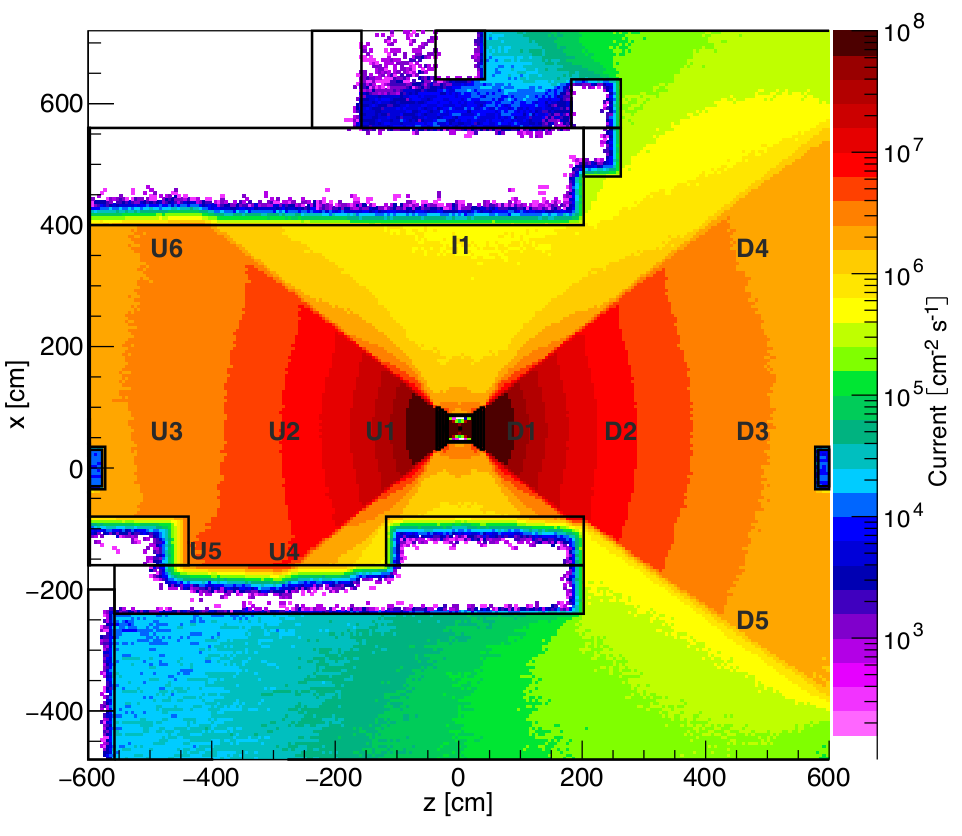
\includegraphics[width = \plotwidth]{fig/chapt5/GIFpp-gCurrent-XZ.png}\\
					\caption{\label{fig:GIFpp-gCurrent:XZ}}
				\end{subfigure}
				\begin{subfigure}{\linewidth}
				    \centering
					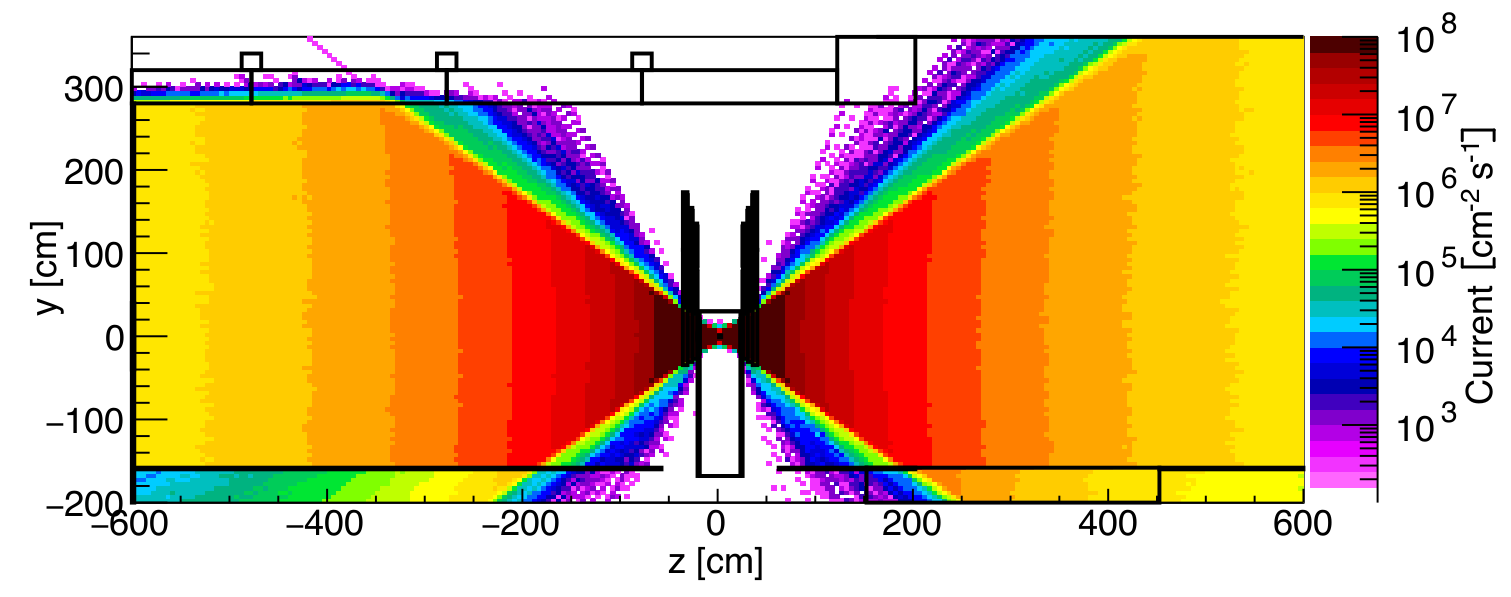
\includegraphics[width = \plotwidth]{fig/chapt5/GIFpp-gCurrent-YZ.png}
					\caption{\label{fig:GIFpp-gCurrent:YZ}}
				\end{subfigure}
				\caption{\label{fig:GIFpp-gCurrent} Simulated unattenuated current of photons in the xz plane (Figure~\ref{fig:GIFpp-gCurrent:XZ}) and yz plane (Figure~\ref{fig:GIFpp-gCurrent:YZ}) through the source at $x=$\SI{0.65}{m} and $y=$\SI{0}{m}. With angular correction filters, the current of \SI{662}{keV} photons is made uniform in xy planes.}
		    \end{figure}
			
			 The source is situated in the muon beam line with the muon beam being available a few times a year. The H4 beam, composed of muons with a momentum of about \SI{150}{GeV/c}, passes through the GIF++ zone and is used to study the performance of the detectors. Its flux is of \SI{104}{particles/s/\square\cm} focused in an area similar to \SIsurface{10}{10}{\cm}. Therefore, with properly adjusted filters, one can imitate the HL-LHC background and study the performance of muon detectors with their trigger/readout electronics in HL-LHC environment.\\

%****************************************** PRIMARILY TESTS AT GIF *************************************************************************
\section{Preliminary tests at GIF}
\label{sec:GIFtests}
	%********************************************* GIF SETUP *************************************************************************
	\subsection{\acl{RPC} test setup}
	\label{ssec:RPCSetup}
	
		During summer 2014, preliminary tests have been conducted in the GIF area on a newly produced RE4/2 chamber labelled RE-4-2-BARC-161. This chamber has been placed into a trolley covered with a tent. The position of the RPC inside the tent and of the tent related to the source is described in Figure~\ref{fig:GIFSetup}. To test this CMS RPC, three different absorber settings were used. First of all, measurements were done with fully opened source. Then, to complete this preliminary study, the gamma flux has been attenuated from a factor 2 and a factor 5. The expected gamma flux at the level of our detector will be discussed in subsection~\ref{ssec:gFlux}.

		\begin{figure}[!h]
			\begin{subfigure}{0.5\linewidth}
			    \centering
				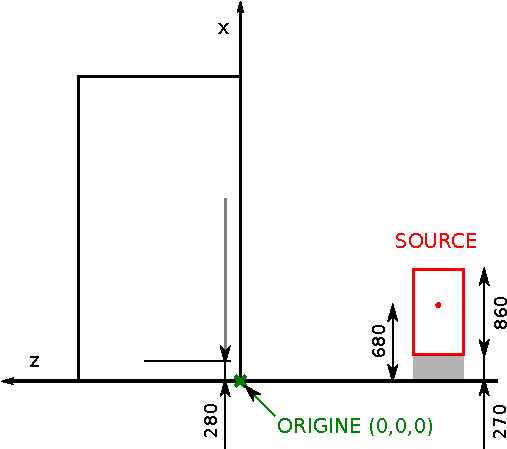
\includegraphics[width = 0.5\plotwidth]{fig/chapt5/GIF-Setup-A.pdf}
				\caption{\label{fig:GIFSetup:A}}
			\end{subfigure}
			\begin{subfigure}{0.5\linewidth}
			    \centering
				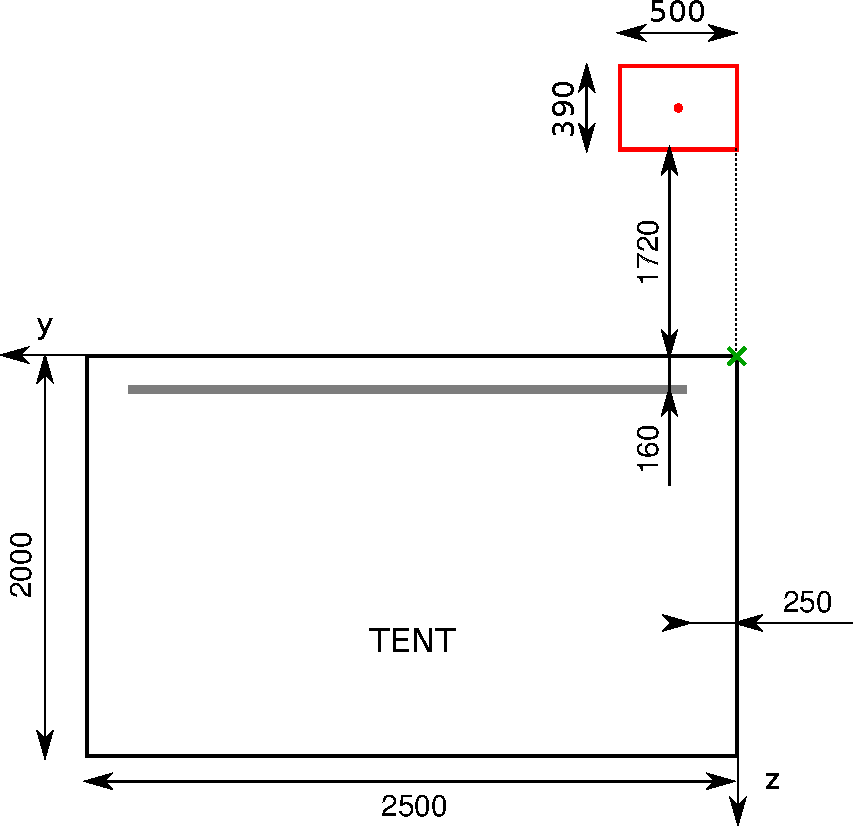
\includegraphics[width = 0.5\plotwidth]{fig/chapt5/GIF-Setup-B.pdf}
				\caption{\label{fig:GIFSetup:B}}
			\end{subfigure}
			\caption{\label{fig:GIFSetup} Description of the RPC setup. Dimensions are given in \si{\mm}. A tent containing RPCs is placed at \SI{1720}{\mm} from the source container. The source is situated in the center of the container. RE-4-2-BARC-161 chamber is \SI{160}{\mm} inside the tent. This way, the distance between the source and the chambers plan is \SI{2060}{\mm}. Figure~\ref{fig:GIFSetup:A} provides a side view of the setup in the $xz$ plane while Figure~\ref{fig:GIFSetup:B} shows a top view in the $yz$ plane.}
		\end{figure}

		\begin{figure}[!h]
			\centering
			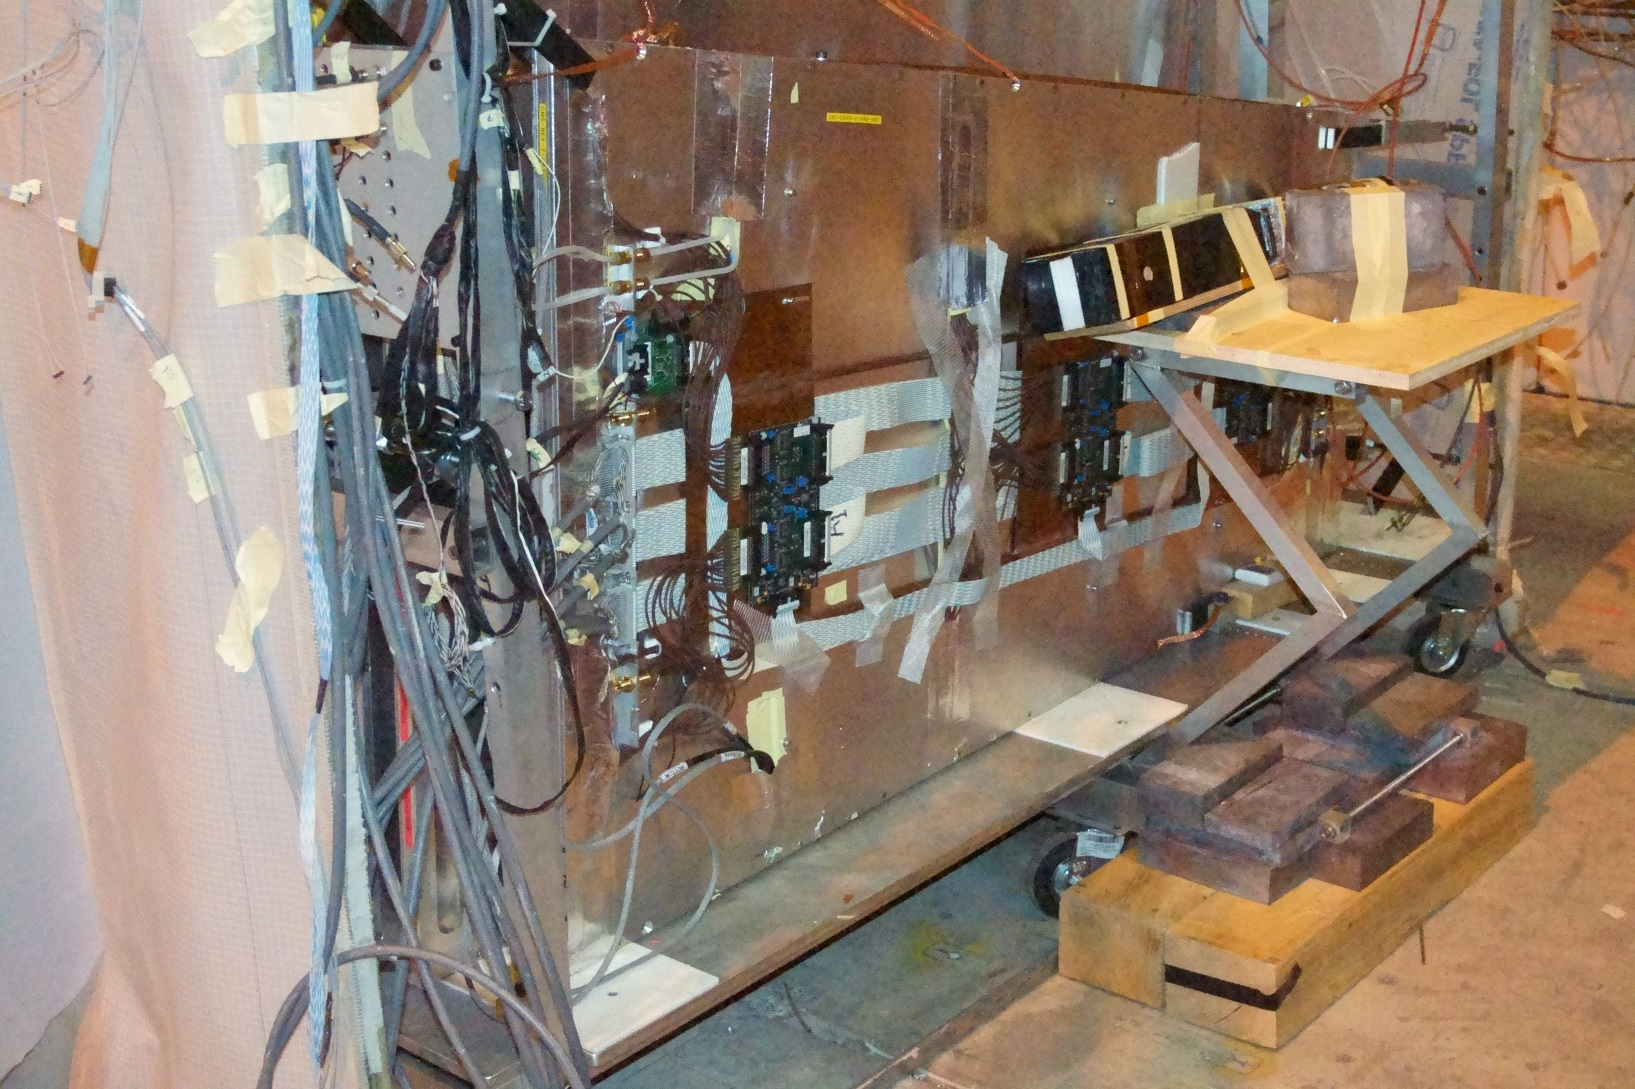
\includegraphics[width = \plotwidth]{fig/chapt5/GIF-RPCSetup.jpg}\\
			\caption{\label{fig:GIF-RPCSetup} RE-4-2-BARC-161 chamber is inside the tent as described in Figure~\ref{fig:GIFSetup}. In the top right, the two scintillators used as trigger can be seen. This trigger system has an inclination of \SI{10}{\degree} relative to horizontal and is placed above half-partition B2 of the RPCs. PMT electronics are shielded thanks to lead blocks placed in order to protect them without stopping photons from going through the scintillators and the chamber.}
		\end{figure}
		
		At the time of the tests, the beam not being operationnal anymore, a trigger composed of 2 plastic scintillators has been placed in front of the setup with an inclination of \SI{10}{\deg} with respect to the detector plane in order to look at cosmic muons. Using this particular trigger layout, shown on Figure~\ref{fig:GIF-RPCSetup}, leads to a cosmic muon hit distribution into the chamber similar to the one in Figure~\ref{fig:HitProf}. Measured without gamma irradiation, two peaks can be seen on the profil of partition B, centered on strips 52 and 59. Section~\ref{ssec:GeoAcc} will help us undertand that these two peaks are due respectively to forward and backward coming cosmic particles where forward coming particles are first detected by the scintillators and then the RPC while the backward coming muons are first detected in the RPC.

		\begin{figure}[!h]
			\centering
			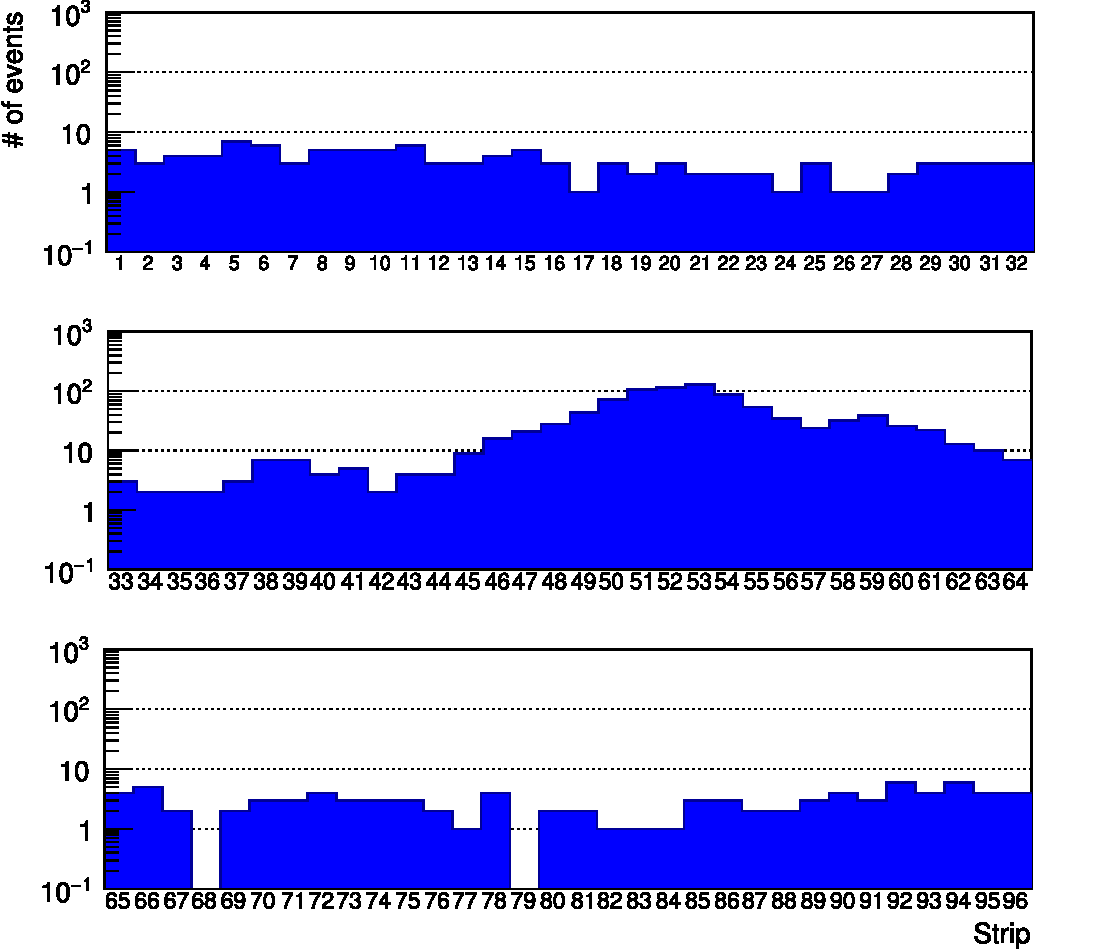
\includegraphics[width = 1.2\plotwidth]{fig/chapt5/Data-21-profile.pdf}\\
			\caption{\label{fig:HitProf} Hit distributions over all 3 parttions of RE-4-2-BARC-161 chamber is showed on these plots. Top, middle and bottom figures respectively correspond to partitions A, B, and C. These plots show that some events still occur in other half-partitions than B2, which corresponds to strips 49 to 64, in front of which the trigger is placed, contributing to the inefficiency of detection of cosmic muons. In the case of partitions A and C, the very low amount of data can be interpreted as noise. On the other hand, it is clear that a little portion of muons reach the half-partition B1, corresponding to strips 33 to 48.}
		\end{figure}
		
	%********************************************** GIF DAQ **************************************************************************
	\subsection{\acl{DAQ}}
	\label{ssec:GIFDAQ}

        As previously described in Section~\ref{ssec:PulseProc}, CMS RPC FEEs provide us with \SI{100}{ns} long LVDS output signals. These signals are then sent into V1190A \acf{TDC} modules manufactured by CAEN~\cite{V1190AMUT}. V1190A are VME units accepting 128 independent Multi-Hit/Multi-Event TDC channels whose signals are treated by 4 \SI{100}{ps} high performance TDC chips, developped by CERN/ECP-MIC Division. The data acquisition used at GIF takes profit of the \textit{Trigger Matching Mode} offered by modules V1190A. A trigger matching is performed in between a trigger time tag and the channel time measurements. The signal provided by the coïncidence of both PMTs is used to trigger the data acquisition. Control over this data acquisition mode, explained through Figure~\ref{fig:V1190A-TMM} is offered through 4 programmable parameters:
        
        \begin{itemize}
            \item \textbf{match window:} the match between a trigger and a hit is done within a programmable time window
            \item \textbf{window offset:} temporal distance between the trigger tag and the start of the trigger matching window
            \item \textbf{extra search margin:} an extended time window is used to ensure that all matching hits are found
            \item \textbf{reject margin:} older hits are automatically rejected to preven buffer overflows and to speed up the search time
        \end{itemize}
        
        \begin{figure}[!h]
			\centering
			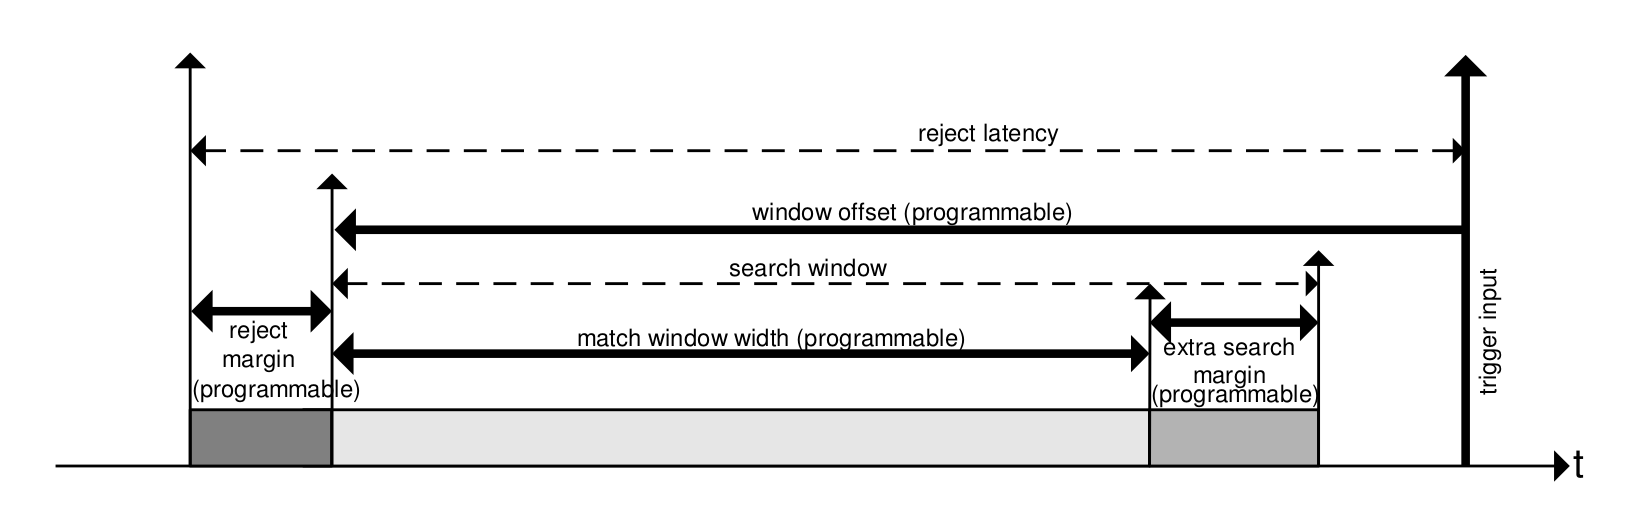
\includegraphics[width = 1.25\plotwidth]{fig/chapt5/V1190A-TMM.png}\\
			\caption{\label{fig:V1190A-TMM} Module V1190A \textit{Trigger Matching Mode} timing diagram.}
		\end{figure}
        
        

	%****************************************** GIF GEOMETRICAL ACCEPTANCE **********************************************************
	\subsection{Geometrical acceptance of the setup layout to cosmic muons}
	\label{ssec:GeoAcc}
				
		In order to profit from a constant gamma irradiation, the detectors inside of the GIF bunker need to be placed in a plane orthogonal to the beam line. The muon beam that used to be available was meant to test the performance of detectors under test. This beam not being active anymore, another solution to test detector performance had to be used. Thus, it has been decided to use cosmic muons detected through a telescope composed of two scintillators. Lead blocks were used as shielding to protect the photomultipliers from gammas as can be seen from Figure~\ref{fig:GIF-RPCSetup}.
					
		An inclination has been given to the cosmic telescope to maximize the muon flux. A good compromise had to be found between good enough muon flux and narrow enough hit distribution to be sure to contain all the events into only one half partitions as required from the limited available readout hardware. Nevertheless, a consequence of the misplaced trigger, that can be seen as a loss of events in half-partition B1 in Figure~\ref{fig:HitProf}, is an inefficiency. Nevertheless, the innefficiency of approximately \SI{20}{\%} highlighted in Figure~\ref{fig:EffCompar} by comparing the performance of chamber BARC-161 in 904 and at GIF without irradiation seems too important to be explained only by the geometrical acceptance of the setup itself. Simulations have been conducted to show how the setup brings inefficiency.
	
		\begin{figure}[!h]
            \centering
			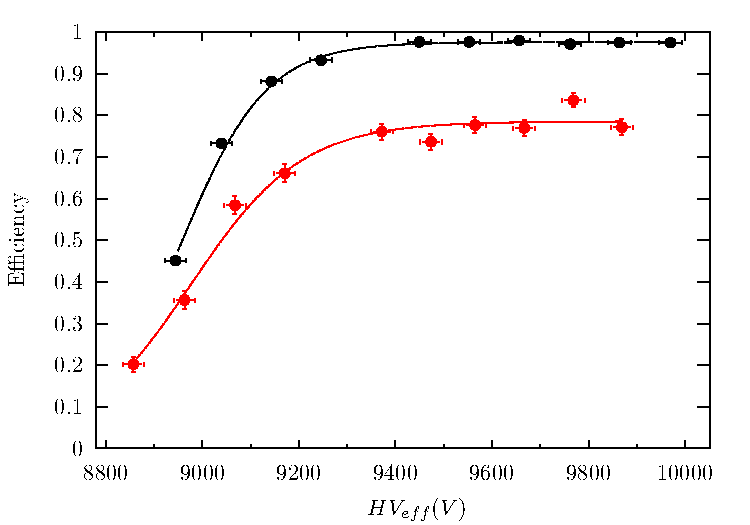
\includegraphics[width = \plotwidth]{fig/chapt5/Eff-Comparison.pdf}
			\caption{\label{fig:EffCompar} Results are derived from data taken on half-partition B2 only. On the 18$^{th}$ of June 2014, data has been taken on chamber RE-2-BARC-161 at building 904 (Prevessin Site) with cosmic muons providing us a reference efficiency plateau of \numerror{97.54}{0.15}\% represented by a black curve. A similar measurement has been done at GIF on the 21$^{st}$ of July with the same chamber giving a plateau of \numerror{78.52}{0.94}\% represented by a red curve.}
		\end{figure}
		
	    %****************************************** SIMULATION LAYOUT *******************************************************
		\subsubsection{Description of the simulation layout}
		\label{sssec:SimLayout}
		
			The layout of GIF setup has been reproduced and incorporated into a \acf{MC} simulation to study the influence of the disposition of the telescope on the final distribution measured by the RPC. A 3D view of the simulated layout is given into Figure~\ref{fig:SimGIFLay}. Muons are generated randomly in a horizontal plane located at a height corresponding to the lowest point of the PMTs. This way, the needed size of the plane in order to simulate events happening at very big azimutal angles (i.e. $\theta\approx\pi$) can be kept relatively small. The muon flux is designed to follow the usual $cos^2\theta$ distribution for cosmic particle. The goal of the simulation is to look at muons that pass through the muon telescope composed of the two scintilators and define their distribution onto the RPC plane. During the reconstruction, the RPC plane is then divided into its strips and each muon track is assigned to a strip.
		
			\begin{figure}[!h]
				\begin{subfigure}{\linewidth}
					\centering
					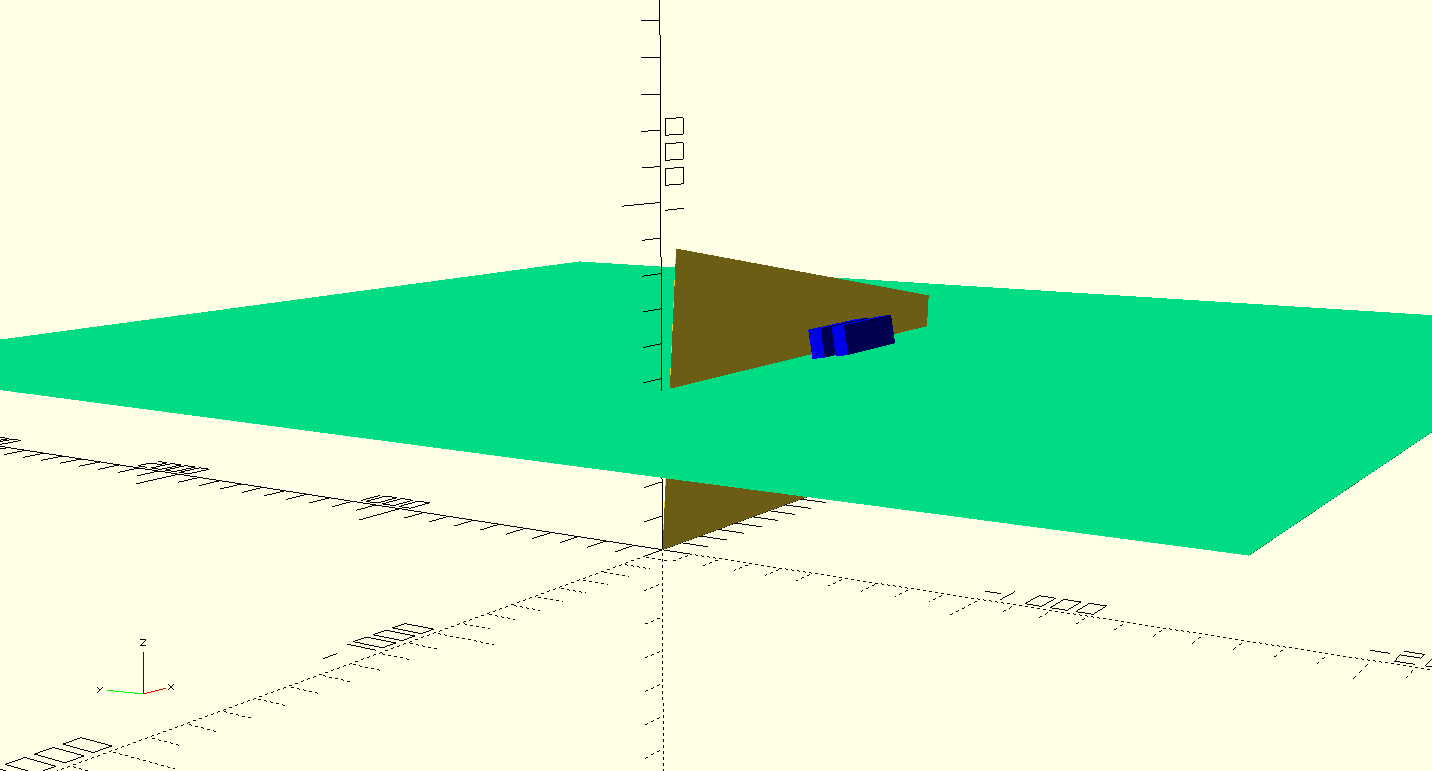
\includegraphics[width = \plotwidth]{fig/chapt5/GIFSetup-SimA.png}\\
					\caption{\label{fig:SimGIFLay:A}}
				\end{subfigure}
				\begin{subfigure}{\linewidth}
					\centering
					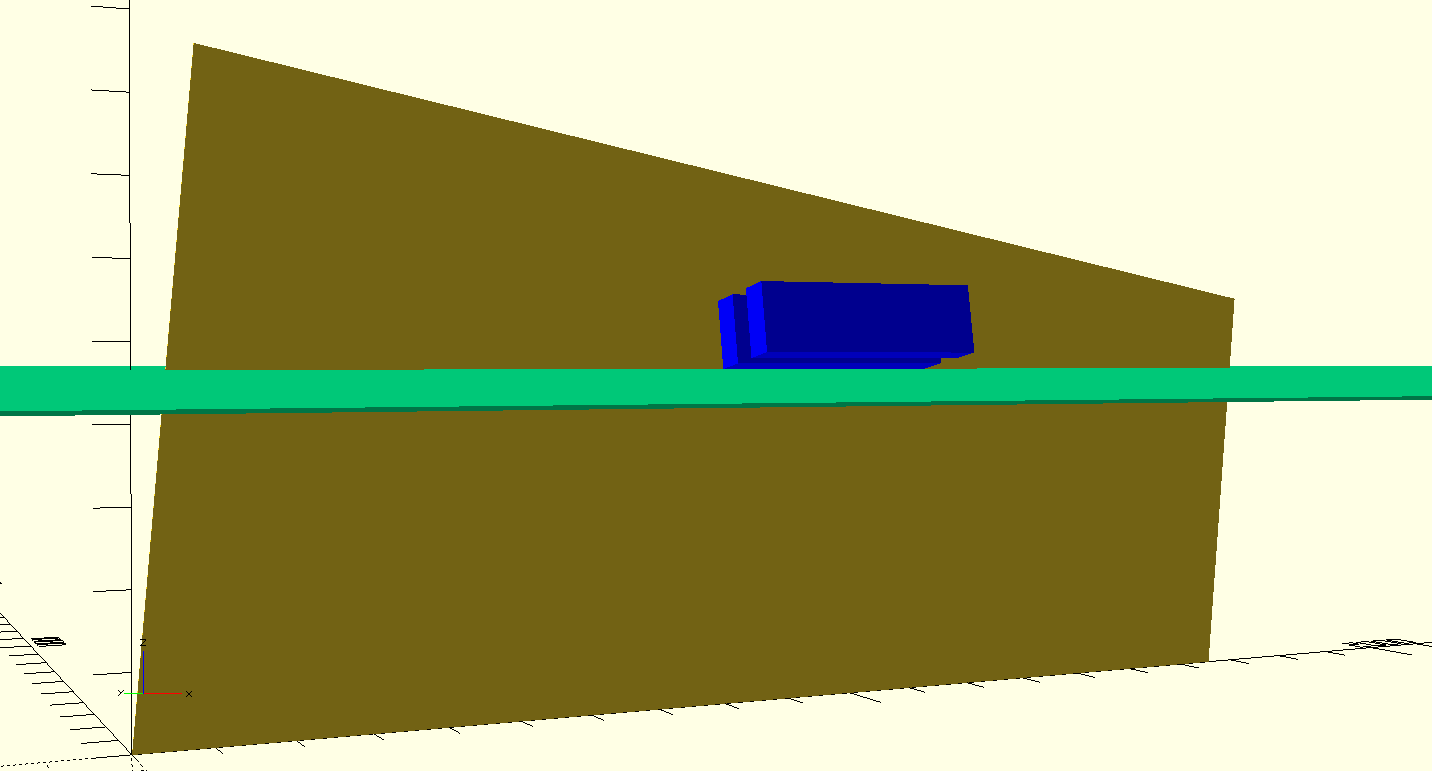
\includegraphics[width = \plotwidth]{fig/chapt5/GIFSetup-SimB.png}
					\caption{\label{fig:SimGIFLay:B}}
				\end{subfigure}
				\caption{\label{fig:SimGIFLay} Representation of the layout used for the simulations of the test setup. The RPC is represented as a yellow trapezoid while the two scintillators as blue cuboids looking at the sky. A green plane corresponds to the muon generation plane within the simulation. Figure~\ref{fig:GIFSetup:A} shows a global view of the simulated setup. Figure~\ref{fig:GIFSetup:B} shows a zommed view that allows to see the 2 scintillators as well as the full RPC plane.}
			\end{figure}
			
			In order to further refine the quality of the simulation and understand deeper the results the dependance of the distribution has been studied for a range of telescope inclinations. Moreover, the threshold applied on the PMT signals has been included into the simulation in the form of a cut. In the approximation of uniform scintillators, it has been considered that the threshold can be understood as the minimum distance particles need to travel through the scintillating material to give a strong enough signal. Particles that travel a distance smaller than the set "threshold" are thus not detected by the telescope and cannot trigger the data taking. Finally, the FEE threshold also has been considered in a similar way. The mean momentum of horizontal cosmic rays is higher than those of vertical ones but the stopping power of matter for momenta ranging from \SI{1}{GeV} to \SI{1}{TeV} stays comparable. It is then possible to assume that the mean number of primary $e^-$/ion pairs per unit length will stay similar and thus, depending on the applied discriminator threshold, muons with the shortest path through the gas volume will deposit less charge and induce a smaller signal on the pick-up strips that could eventually not be detected. These two thresholds also restrain the overall geometrical acceptance of the system.
		
	    %***************************************** SIMULATION PROCEDURE *****************************************************
		\subsubsection{Simulation procedure}
		\label{sssec:SimProc}
		
			The simulation software has been designed using C++ and the output data is saved into ROOT histograms. Simulations start for a threshold $T_{scint}$ varying in a range from 0 to \SI{45}{mm} in steps of \SI{5}{mm}, where $T_{scint}=$ \SI{0}{mm} corresponds to the case where there isn't any threshold apply on the input signal while $T_{scint}=$ \SI{45}{mm}, which is the scintillator thickness, is the case where muons cannot arrive orthogonally onto the scintillator surface. For a given $T_{scint}$, a set of \acs{RPC} thresholds are considered. The RPC threshold, $T_{RPC}$ varies from \SI{2}{mm}, the thickness of the gas volume, to \SI{3}{mm} in steps of \SI{0.25}{mm}. For each ($T_{scint}$;$T_{RPC}$) pair, $N_{\mu}=10^8$ muons are randomly generated inside the muon plane described in the previous paragraph with an azimutal angle $\theta$ chosen to follow a $cos^2\theta$ distribution. 
			
			Planes are associated to each surface of the scintillators. Knowing muon position into the muon plane and its direction allows us, by assuming that muons travel in a straight line, to compute the intersection of the muon track with these planes. Applying conditions to the limits of the surfaces of the scintillator faces then gives us an answer to weither or not the muon passed through the scintillators. In the case the muon has indeed passed through the telescope, the path through each scintillator is computed and muons whose path was shorter than $T_{scint}$ are rejected and are thus considered as having not interacted with the setup.
			
			On the contrary, if the muon is labeled as good, its position within the RPC plane is computed and the corresponding strip, determined by geometrical tests in the case the distance through the gas volume was enough not to be rejected because of $T_{RPC}$, gets a hit and several histograms are filled in order to keep track of the generation point on the muon plane, the intersection points of the reconstructed muons within the telescope, or on the RPC plane, the path traveled through each individual scintillator or the gas volume, as well as other histograms. Moreover, muons fill different histograms weither they are forward or backward coming muons. They are discriminated according to their direction components. When a muon is generated, an $(x,y,z)$ position is assigned into the muon plane as well as a ($\theta$;$\phi$) pair that gives us the direction it's coming from. This way, muons satisfying the condition $0\leq\phi<\pi$ are designated as backward coming muons while muons satisfying $\pi\leq\phi<2\pi$ as forward coming muons.
			
			This simulation is then repeated for different telescope inclinations ranging in between 4 and \SI{20}{\degree} and varying in steps of \SI{2}{\degree}. Due to this inclination and to the vertical position of the detector under test, the muon distribution reconstructed in the detector plane is asymmetrical. The choice as been made to chose a skew distribution formula to fit the data built as the multiplication of gaussian and sigmoidal curves together. A typical gaussian formula is given as ~\ref{for:gaus} and has three free parameters as $A_g$, its amplitude, $\bar{x}$, its mean value and $\sigma$, its root mean square. Sigmoidal curves as given by formula~\ref{for:sigm} are functions converging to $0$ and $A_s$ as $x$ diverges. The inflexion point is given as $x_i$ and $\lambda$ is proportional to the slope at $x = x_i$. In the limit where $\lambda\longrightarrow\infty$, the sigmoid becomes a step function.
			
			\begin{center}
				\begin{equation}
				\label{for:gaus}
					g(x) = A_g e^{\frac{-(x-\bar{x})^2}{2\sigma^2}}
				\end{equation}
			\end{center}
			
			\begin{center}
				\begin{equation}
				\label{for:sigm}
					s(x) = \frac{A_s}{1+e^{-\lambda(x-x_i)}}
				\end{equation}
			\end{center}
			
		Finally, a possible representation of a skew distribution is given by formula~\ref{for:skew} and is the product of \ref{for:gaus} and \ref{for:sigm}. Naturally, here $A_{sk} = A_g \times A_s$ and represents the theoretical maximum in the limit where the skew tends to a gaussian function.
			
			\begin{center}
				\begin{equation}
				\label{for:skew}
					sk(x) = g(x)\times s(x) = A_{sk}\frac{e^{\frac{-(x-\bar{x})^2}{2\sigma^2}}}{1+e^{-\lambda(x-x_i)}}
				\end{equation}
			\end{center}
		
	    %***************************************** SIMULATION RESULTS *******************************************************
		\subsubsection{Results}
		\label{sssec:SimRes}
			
			\paragraph{Influence of $\mathbf{T_{scint}}$ on the muon distribution}
			
			\paragraph{Influence of $\mathbf{T_{RPC}}$ on the muon distribution}
		
			\paragraph{Influence of the telescope inclination on the muon distribution}
			
			\paragraph{Comparison to data taken at GIF without irradiation}
		
	%****************************************** PHOTON FLUX AT GIF ******************************************************************
	\subsection{Photon flux at \acs{GIF}}
	\label{ssec:gFlux}
			
		%****************************************** EXPECTATIONS FROM SIMULATIONS ********************************************
		\subsubsection{Expectations from simulations}
		\label{sssec:Simulations}
		
			In order to understand and evaluate the $\gamma$ flux in the GIF area, simulations had been conducted in 1999 and published by S. Agosteo et al ~\cite{AGOSTEO1999}. Table~\ref{tab:Sim1997} presented in this article gives us the $\gamma$ flux for different distances $D$ to the source. This simulation was done using GEANT and a \acf{MCNP} transport code, and the flux $F$ is given in number of $\gamma$ per unit area and unit time along with the estimated error from these packages expressed in \%.
			
			\begin{table}[!h]
				\hspace*{-1.1cm}
				\begin{tabular}{|*{5}{c|}}
					\hline
					Nominal & \multicolumn{4}{c|}{Photon flux $F$ [\si{\second^{-1}\cm^{-2}}]} \\
					\cline{2-5}
					ABS & at $D$ = \SI{50}{\cm} & at $D$ = \SI{155}{\cm} & at $D$ = \SI{300}{\cm} & at $D$ = \SI{400}{\cm} \\
					\hline
					1 & $0.12 \cdot 10^8 \pm 0.2\%$ & $0.14 \cdot 10^7 \pm 0.5\%$ & $0.45 \cdot 10^6 \pm 0.5\%$ & $0.28 \cdot 10^6 \pm 0.5\%$ \\
					\hline
					2 & $0.68 \cdot 10^7 \pm 0.3\%$ & $0.80 \cdot 10^6 \pm 0.8\%$ & $0.25 \cdot 10^6 \pm 0.8\%$ & $0.16 \cdot 10^6 \pm 0.6\%$ \\
					\hline
					5 & $0.31 \cdot 10^7 \pm 0.4\%$ & $0.36 \cdot 10^6 \pm 1.2\%$ & $0.11 \cdot 10^6 \pm 1.2\%$ & $0.70 \cdot 10^5 \pm 0.9\%$ \\
					\hline
				\end{tabular}
				\caption{\label{tab:Sim1997} Total photon flux ($E\gamma \leq$ \SI{662}{\keV}) with statistical error predicted considering a $^{137}$Cs activity of \SI{740}{\GBq} at different values of the distance $D$ to the source along the x-axis of irradiation field~\cite{AGOSTEO1999}.}
			\end{table}
			
			\begin{figure}[!h]
				\centering
				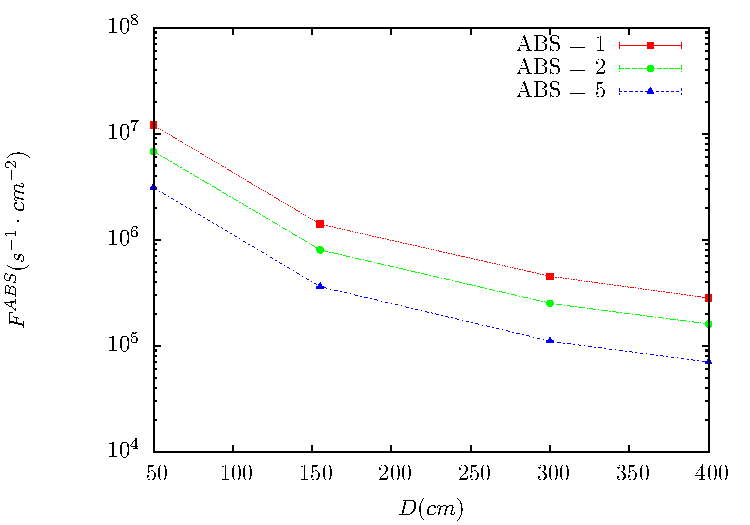
\includegraphics[width = \plotwidth]{fig/chapt5/simulated_flux.pdf}\\
				\caption{\label{fig:Sim1997} $\gamma$ flux $F(D)$ is plot using values from table~\ref{tab:Sim1997}. As expected, the plot shows similar attenuation behaviours with increasing distance for each absorption factors.}
			\end{figure}
			
			The simulation doesn't directly provides us with an estimated flux at the level of our RPC. First of all, it is needed to extract the value of the flux from the available data contained in the original paper and then to estimate the flux in 2014 at the time the experimentation took place. Figure~\ref{fig:Sim1997} that contains the data from Table~\ref{tab:Sim1997}. In the case of a pointlike source emiting isotrope and homogeneous gamma radiations, the gamma flux $F$ at a distance $D$ to the source with respect to a reference point situated at $D_0$ where a known flux $F_0$ is measured will be expressed like in Equation~\ref{eq:Flux}, assuming that the flux decreases as $1/D^2$, where $c$ is a fitting factor.
			
			\begin{equation}
				F^{ABS} = F_0^{ABS} \times \left( \frac{c D_0}{D} \right)^2
				\label{eq:Flux}
			\end{equation}
			
			By rewriting Equation~\ref{eq:Flux}, it comes that :
			
			\begin{eqnarray}
				c & = & \frac{D}{D_0}\sqrt{\frac{F^{ABS}}{F_0^{ABS}}}\label{eq:Factor}\\
				\Delta c & = & \frac{c}{2}\left(\frac{\Delta F^{ABS}}{F^{ABS}}+\frac{\Delta F^{ABS}_0}{F^{ABS}_0}\right)\label{eq:FactorErr}
			\end{eqnarray}
			
			Finally, using Equation~\ref{eq:Factor} and the data in Table~\ref{tab:Sim1997} with $D_0=$ \SI{50}{cm} as reference point, we can build Table~\ref{tab:CorrFactor}. It is interesting to note that $c$ for each value of $D$ doesn't depend on the absorption factor.
			
			\begin{table}[!h]
				\centering
				\begin{tabular}{|*{4}{c|}}
					\hline
					Nominal & \multicolumn{3}{c|}{Correction factor $c$} \\
					ABS & at $D$ = \SI{155}{\cm} & at $D$ = \SI{300}{\cm} & at $D$ = \SI{400}{\cm} \\
					\hline
					1 & $1.059 \pm 0.70\%$ & $1.162 \pm 0.70\%$ & $1.222 \pm 0.70\%$ \\
					\hline
					2 & $1.063 \pm 1.10\%$ & $1.150 \pm 1.10\%$ & $1.227 \pm 0.90\%$ \\
					\hline
					5 & $1.056 \pm 1.60\%$ & $1.130 \pm 1.60\%$ & $1.202 \pm 1.30\%$ \\
					\hline
				\end{tabular}
				\caption{\label{tab:CorrFactor} Correction factor c is computed thanks to formulae~\ref{eq:Factor} taking as reference $D_0 =$ \SI{50}{cm} and the associated flux $F_0^{ABS}$ for each absorption factor available in table~\ref{tab:Sim1997}.}
			\end{table}
			
			For the range of $D/D_0$ values available, it is possible to use a simple linear fit to get the evolution of $c$. The linear fit will then use only 2 free parameters, $a$ and $b$, as written in Equation~\ref{eq:LinearApprox}. This gives us the results showed in Figure~\ref{fig:CorrFactor}. Figure~\ref{fig:CorrFactor:B} confirms that using only a linear fit to extract $c$ is enough as the evolution of the rate that can be obtained superimposes well on the simulation points.
			
			\begin{eqnarray}
				c\left(\frac{D}{D_0}\right) & = & a\frac{D}{D_0} + b\label{eq:LinearApprox}\\
				F^{ABS} & = & F^{ABS}_0 \left( a + \frac{bD_0}{D} \right)^2\label{eq:FluxLinearAp}\\
				\Delta F^{ABS} & = & F^{ABS} \left[\frac{\Delta F^{ABS}_0}{F^{ABS}_0} + 2\frac{\Delta a + \Delta b\frac{D_0}{D}}{a + \frac{bD_0}{D}}\right]\label{eq:FluxLinearApErr}
			\end{eqnarray}
			
			\begin{figure}[!h]
				\begin{subfigure}{\linewidth}
					\centering
					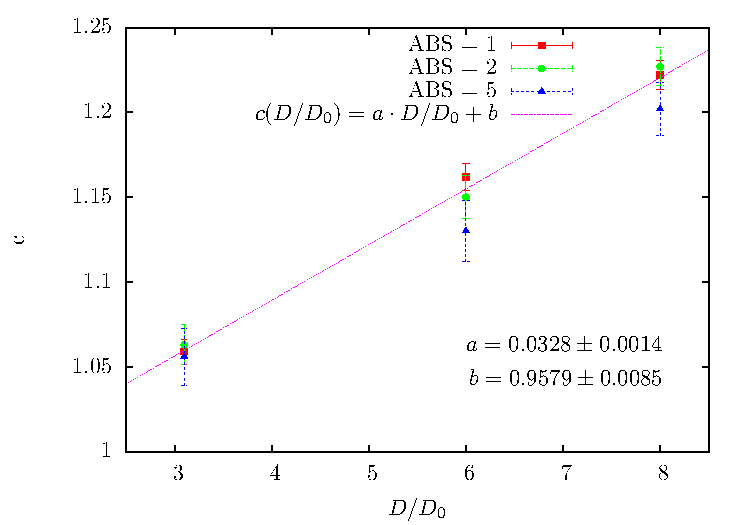
\includegraphics[width = \plotwidth]{fig/chapt5/flux_correction.pdf}\\
					\caption{\label{fig:CorrFactor:A}}
				\end{subfigure}
				\begin{subfigure}{\linewidth}
					\centering
					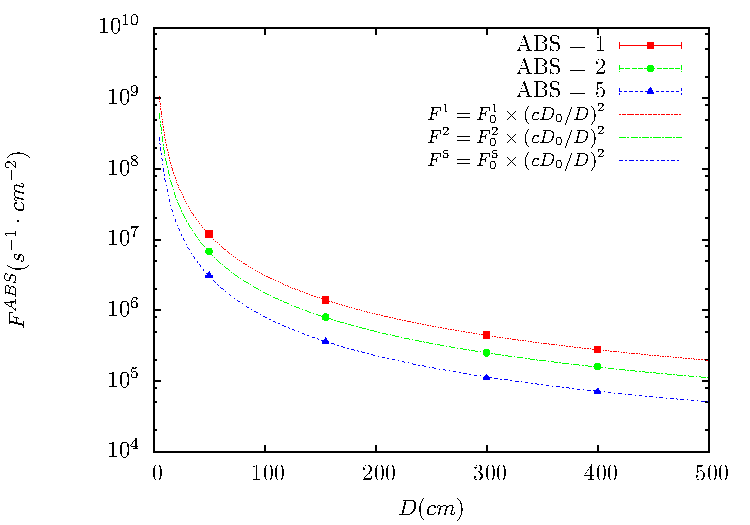
\includegraphics[width = \plotwidth]{fig/chapt5/correction_model.pdf}
					\caption{\label{fig:CorrFactor:B}}
				\end{subfigure}
				\caption{\label{fig:CorrFactor} Figure~\ref{fig:CorrFactor:A} shows the linear approximation fit done via formulae~\ref{eq:LinearApprox} on data from table~\ref{tab:CorrFactor}. Figure~\ref{fig:CorrFactor:B} shows a comparison of this model with the simulated flux using a and b given in figure~\ref{fig:CorrFactor:A} in formulae ~\ref{eq:Flux} and the reference value $D_0 = 50 cm$ and the associated flux for each absorption factor $F_0^{ABS}$ from table~\ref{tab:Sim1997}}
			\end{figure}
			
			In the case of the 2014 GIF tests, the RPC plane is located at a distance $D=$\SI{206}{cm} to the source. Moreover, to estimate the strength of the flux in 2014, it is necessary to consider the nuclear decay through time assiciated to the Cesium source whose half-life is well known ($t_{1/2}=$ \SIerror{30.05}{0.08}{y}). The very first source activity measurement has been done on the $5^{th}$ of March 1997 while the GIF tests where done in between the $20^{th}$ and the $31^{st}$ of August 2014, i.e. at a time $t=$ \SIerror{17.47}{0.02}{y} resulting in an attenuation of the activity from \SI{740}{GBq} in 1997 to \SI{494}{GBq} in 2014. All the needed information to extrapolate the flux through our detector in 2014 has now been assembled, leading to the Table~\ref{tab:extra2014}. It isinteresting to note that for a common RPC sensitivity to $\gamma$ of $2 \cdot 10^{-3}$, the order of magnitude of the estimated hit rate per unit area is of the order of the \si{kHz} for the fully opened source. Moreover, taking profit of the two working absorbers, it will be possible to scan background rates at \SI{0}{Hz}, $\sim$\SI{300}{Hz} as well as $\sim$\SI{600}{Hz}. Without source, a good estimate of the intrinsic performance will be available. Then at \SI{300}{Hz}, the goal will be to show that the detectors fulfill the performance certification of CMS RPCs. Then a first idea of the performance of the detectors at higher background will be provided with absorbtion factors 2 ($\sim$\SI{600}{Hz}) and 1 (no absorbtion). \textbf{\textit{[Here I will also put a reference to the plot showing the estimated background rate at the level of RE3/1 in the case of HL-LHC but this one being in another chapter, I will do it later.]}}
			
			\begin{table}[!h]
				\hspace*{-2cm}
				\begin{tabular}{|*{5}{c|}}
					\hline
					Nominal & \multicolumn{3}{c|}{Photon flux $F$ [\si{\second^{-1}\cm^{-2}}]} & Hit rate/unit area [\si{Hz.cm^{-2}}] \\
					ABS & at $D_0^{1997}$ = \SI{50}{\cm} & at $D^{1997}$ = \SI{206}{\cm} & at $D^{2014}$ = \SI{206}{\cm} & at $D^{2014}$ = \SI{206}{\cm} \\
					\hline
					1 & $0.12 \cdot 10^8 \pm 0.2\%$ & $0.84 \cdot 10^6 \pm 0.3\%$ & $0.56 \cdot 10^6 \pm 0.3\%$ & $1129 \pm 32$ \\
					\hline
					2 & $0.68 \cdot 10^7 \pm 0.3\%$ & $0.48 \cdot 10^6 \pm 0.3\%$ & $0.32 \cdot 10^6 \pm 0.3\%$ & $640 \pm 19$ \\
					\hline
					5 & $0.31 \cdot 10^7 \pm 0.4\%$ & $0.22 \cdot 10^6 \pm 0.3\%$ & $0.15 \cdot 10^6 \pm 0.3\%$ & $292 \pm 9$ \\
					\hline
				\end{tabular}
				\caption{\label{tab:extra2014} The data at $D_0$ in 1997 is taken from~\cite{AGOSTEO1999}. In a second step, using Equations~\ref{eq:FluxLinearAp} and~\ref{eq:FluxLinearApErr}, the flux at $D$ can be estimated in 1997. Then, taking into account the attenuation of the source activity, the flux at $D$ can be estimated at the time of the tests in GIF in 2014. Finally, assuming a sensitivity of the RPC to $\gamma$ $s = 2 \cdot 10^{-3}$, an estimation of the hit rate per unit area is obtained.}
			\end{table}

		%****************************************** DOSE MEASUREMENTS ********************************************************
		\subsubsection{Dose measurements}
		\label{sssec:Dose}
			
			\begin{figure}[!h]
				\centering
				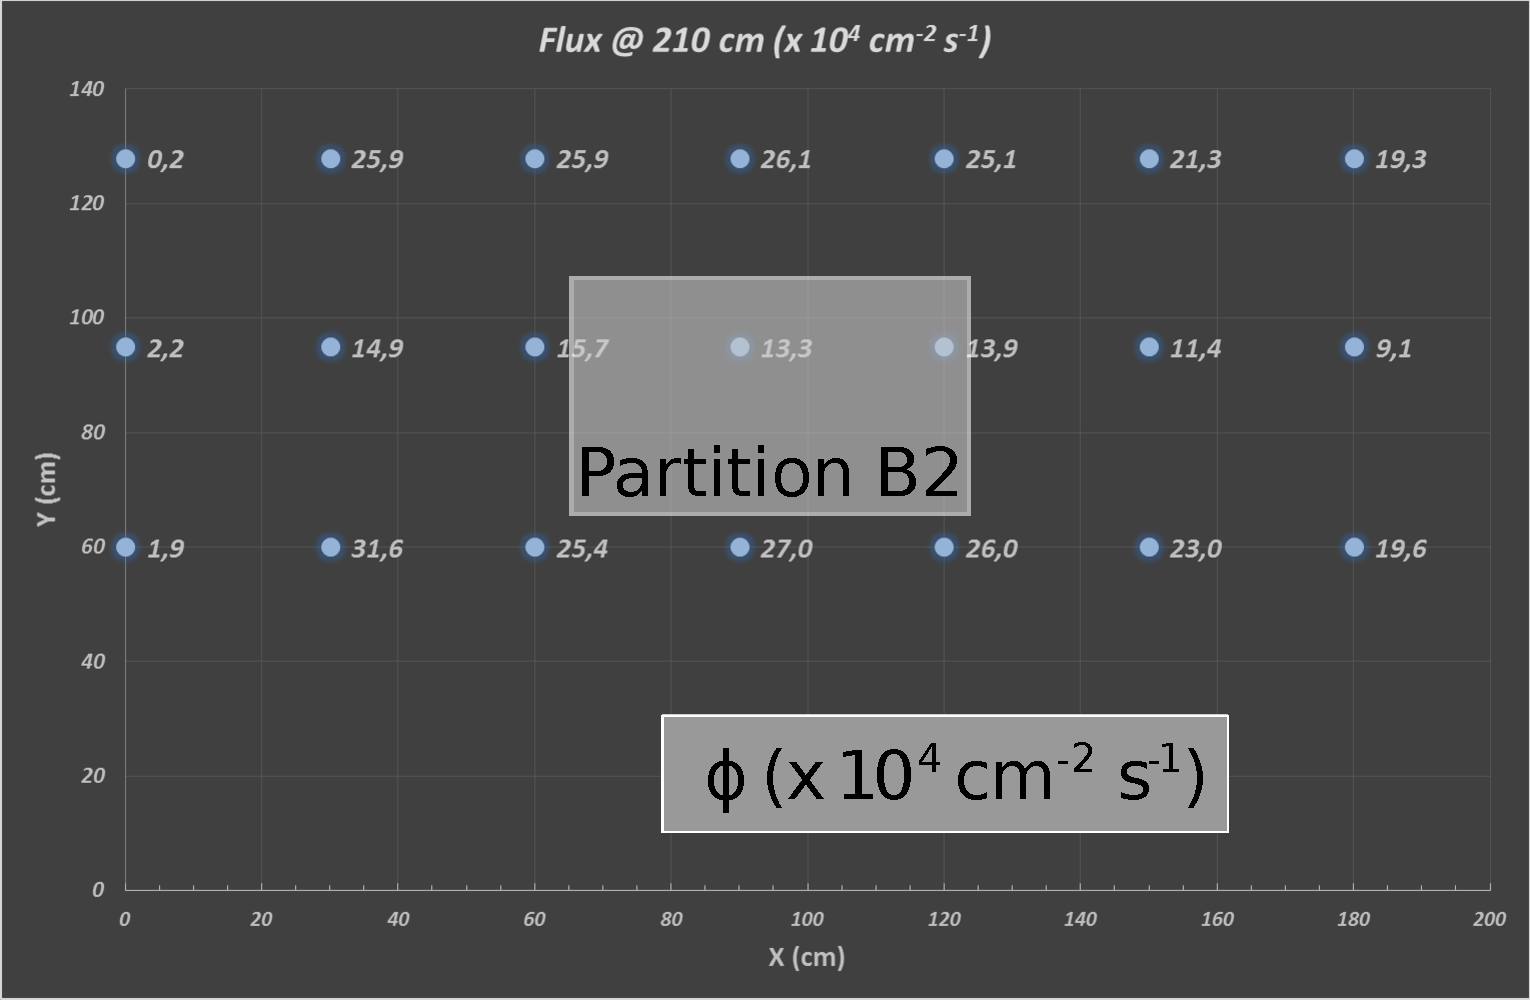
\includegraphics[width = \plotwidth]{fig/chapt5/GIF-fluxes.pdf}\\
				\caption{\label{fig:Dose} Dose measurements has been done in a plane corresponding to the tents front side. This plan is \SI{1900}{\mm} away from the source. As explained in the first chapter, a lens-shaped lead filter provides a uniform photon flux in the vertical plan orthogonal to the beam direction. If the second line of measured fluxes is not taken into account because of lower values due to experimental equipments in the way between the source and the tent, the uniformity of the flux is well showed by the results.}
			\end{figure}

    %************************************* GIF PRELIMINARY RESULTS ******************************************************************
	\subsection{Results and discussions}
	\label{ssec:results6}
		
		\begin{figure}[!h]
			\begin{subfigure}{0.5\linewidth}
				\centering
				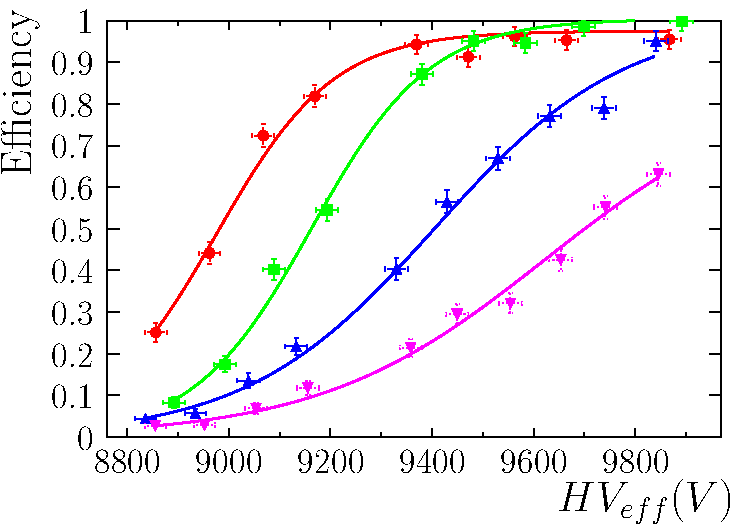
\includegraphics[width = 0.6\plotwidth]{fig/chapt5/Efficiencies.pdf}
				\caption{\label{fig:GIFResults:E}}
			\end{subfigure}
			\begin{subfigure}{0.5\linewidth}
				\centering
				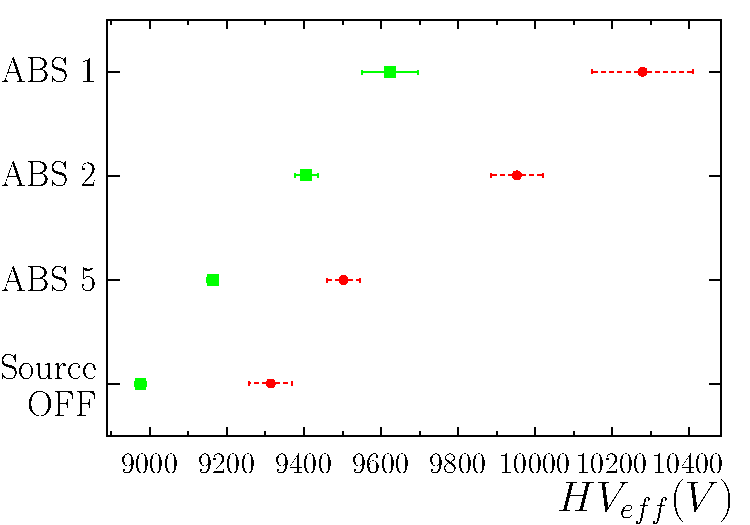
\includegraphics[width = 0.6\plotwidth]{fig/chapt5/Evol_HV.pdf}\\
				\caption{\label{fig:GIFResults:WP}}
			\end{subfigure}
			\begin{subfigure}{0.5\linewidth}
				\centering
				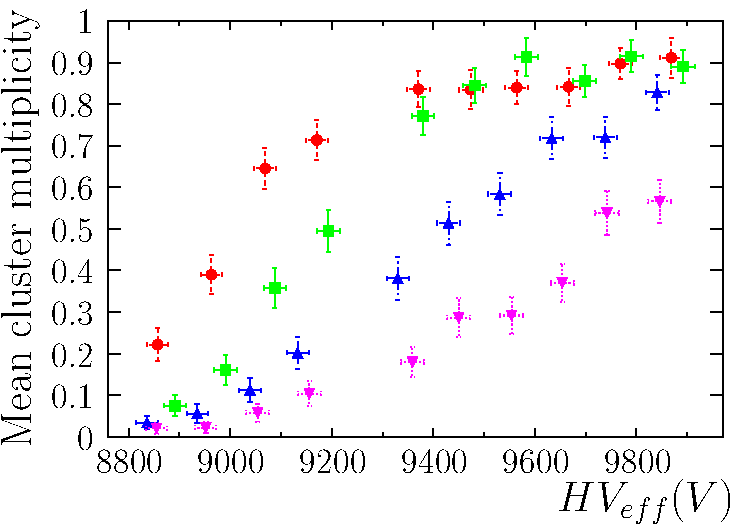
\includegraphics[width = 0.6\plotwidth]{fig/chapt5/Clustermultiplicities.pdf}
				\caption{\label{fig:GIFResults:CM}}
			\end{subfigure}
			\begin{subfigure}{0.5\linewidth}
				\centering
				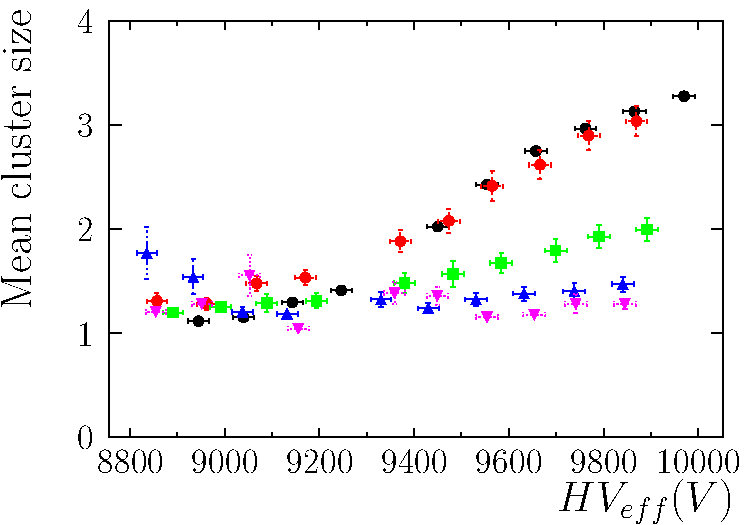
\includegraphics[width = 0.6\plotwidth]{fig/chapt5/Clustersizes.pdf}\\
				\caption{\label{fig:GIFResults:CS}}
			\end{subfigure}
			\caption{\label{fig:GIFResults} }
		\end{figure}

%****************************************** CONSOLIDATION TESTS AT GIF++ *******************************************************************
\newpage

\section{Longevity tests at \acs{GIF++}}
\label{sec:GIFtests}

    Longevity studies imply a monitoring of the performance of the detectors probed using a high intensity muon beam in a irradiated environment by periodically measuring their rate capability, the dark current running through them and the bulk resistivity of the Bakelite composing their electrodes. GIF++, with its very intense $^{137}$Cs source, provides the perfect environment to perform such kind of tests. Assuming a maximum acceleration factor of 3, it is expected to accumulate the equivalent charge in 1.7 years.\\
    As the maximum background is found in the endcap, the choice naturally was made to focus the GIF++ longevity studies on endcap chambers. Most of the RPC system was installed in 2007. Nevertheless, the large chambers in the fourth endcap (RE4/2 and RE4/3) have been installed during LS1 in 2014. The Bakelite of these two different productions having different properties, four spare chambers of the present system were selected, two RE2,3/2 spares and two RE4/2 spares. Having two chambers of each type allows to always keep one of them non irradiated as reference, the performance evolution of the irradiated chamber being then compared through time to the performance of the non irradiated one.\\
    The performance of the detectors under different level of irradiation is measured periodically during dedicated test beam periods using the H4 muon beam. In between these test beam periods, the two RE2,3/2 and RE4/2 chambers selected for this study are irradiated by the $^{137}$Cs source in order to accumulate charge and the gamma background is monitored, as well as the currents. The two remaining chambers are kept non-irradiated as reference detectors. Due to the limited gas flow in GIF++, the RE4 chamber remained non-irradiated until end of November 2016 where a new mass flow controller has been installed allowing for bigger volumes of gas to flow in the system.\\
     Figures~\ref{Fig:Eff-vs-Rate} and \ref{Fig:WP-vs-Rate} give us for different test beam periods, and thus for increasing integrated charge through time, a comparison of the maximum efficiency, obtained using a sigmoid-like function, and of the working point of both irradiated and non irradiated chambers~\cite{SIGMOID2005}. No aging is yet to see from this data, the shifts in $\gamma$ rate per unit area  in between irradiated and non irradiated detectors and RE2 and RE4 types being easily explained by a difference of sensitivity due to the various Bakelite resistivities of the HPL electrodes used for the electrode production.\\
     Collecting performance data at each test beam period allows us to extrapolate the maximum efficiency for a background hit rate of \SI{300}{Hz/cm^2} corresponding to the expected HL-LHC conditions. Aging effects could emerge from a loss of efficiency with increasing integrated charge over time, thus Figure~\ref{Fig:Eff-vs-Qint} helps us understand such degradation of the performance of irradiated detectors in comparison with non irradiated ones. The final answer for an eventual loss of efficiency is given in Figure~\ref{Fig:Eff-Bef-Aft} by comparing for both irradiated and non irradiated detectors the efficiency sigmoids before and after the longevity study. Moreover, to complete the performance information, the Bakelite resistivity is regularly measured thanks to $Ag$ scans (Figure~\ref{Fig:Res-vs-Qint}) and the noise rate is monitored weekly during irradiation periods (Figure~\ref{Fig:Noise-vs-Qint}). At the end of 2016, no signs of aging were observed and further investigation is needed to get closer to the final integrated charge requirements proposed for the longevity study of the present CMS RPC sub-system.\\
    
    
    \begin{figure}[!h]
    	\begin{subfigure}{0.5\linewidth}
			\centering
    		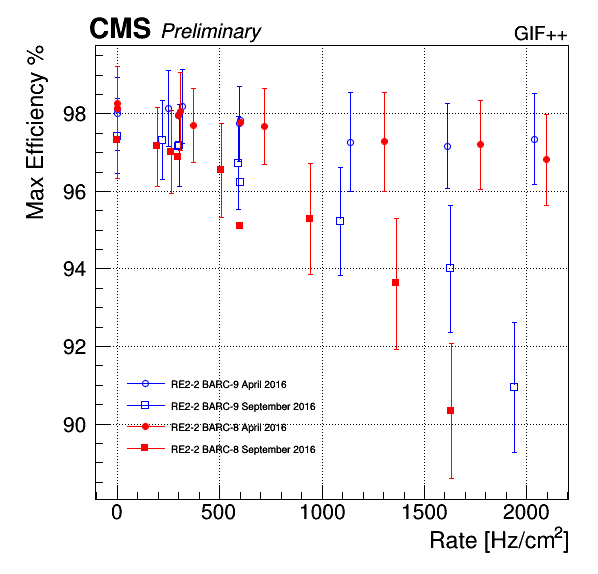
\includegraphics[width=\linewidth]{fig/chapt5/Eff-vs-Rate-RE2.png}\\
        	\caption{\label{Fig:Eff-vs-Rate:RE2}}
    	\end{subfigure}
    	\begin{subfigure}{0.5\linewidth}
			\centering
    		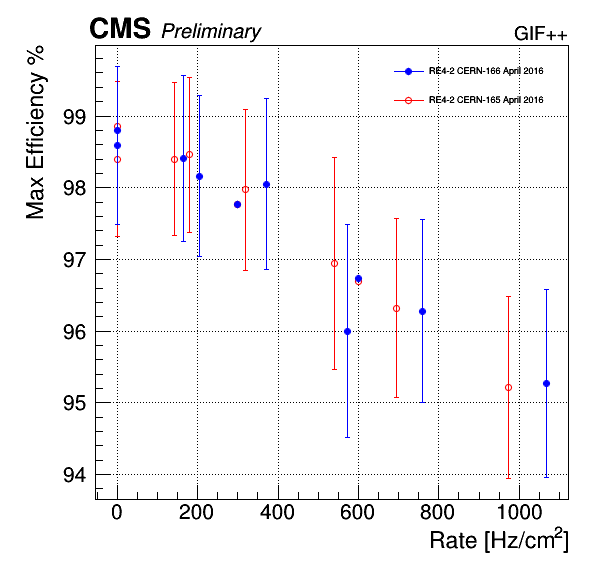
\includegraphics[width=\linewidth]{fig/chapt5/Eff-vs-Rate-RE4.png}\\
        	\caption{\label{Fig:Eff-vs-Rate:RE4}}
    	\end{subfigure}
        \caption{\label{Fig:Eff-vs-Rate} Evolution of the maximum efficiency for RE2 (\ref{Fig:Eff-vs-Rate:RE2}) and RE4 (\ref{Fig:Eff-vs-Rate:RE4}) chambers with increasing extrapolated $\gamma$ rate per unit area at working point. Both irradiated (blue) and non irradiated (red) chambers are shown.}
    \end{figure}
    
    \begin{figure}[!h]
    	\begin{subfigure}{0.5\linewidth}
			\centering
    		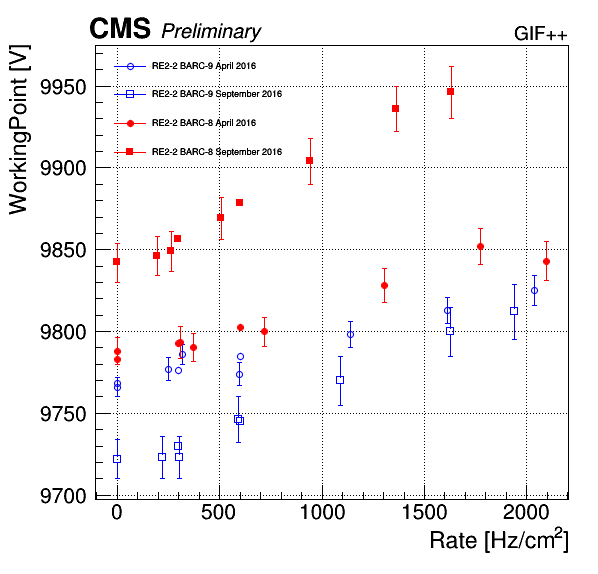
\includegraphics[width=\linewidth]{fig/chapt5/WP-vs-Rate-RE2.png}\\
        	\caption{\label{Fig:WP-vs-Rate:RE2}}
    	\end{subfigure}
    	\begin{subfigure}{0.5\linewidth}
			\centering
    		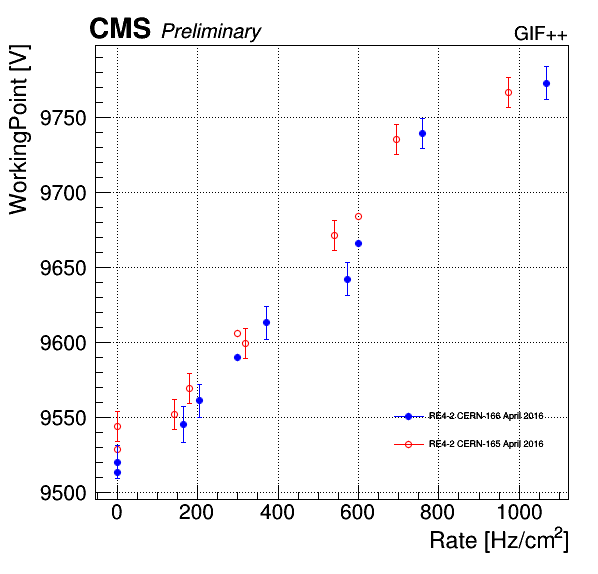
\includegraphics[width=\linewidth]{fig/chapt5/WP-vs-Rate-RE4.png}\\
        	\caption{\label{Fig:WP-vs-Rate:RE4}}
    	\end{subfigure}
        \caption{\label{Fig:WP-vs-Rate} Evolution of the working point for RE2 (\ref{Fig:WP-vs-Rate:RE2}) and RE4 (\ref{Fig:WP-vs-Rate:RE4}) with increasing extrapolated $\gamma$ rate per unit area at working point. Both irradiated (blue) and non irradiated (red) chambers are shown.}
    \end{figure}
    
    \begin{figure}[!h]
    	\begin{subfigure}{0.5\linewidth}
			\centering
    		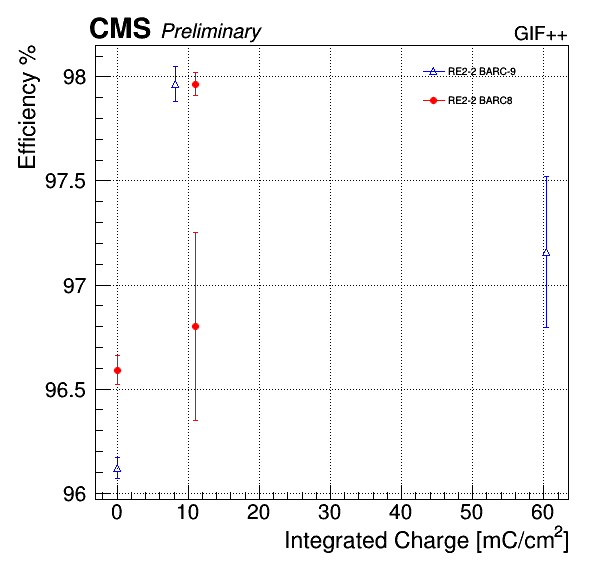
\includegraphics[width=\linewidth]{fig/chapt5/Eff-vs-Qint-RE2.png}\\
        	\caption{\label{Fig:Eff-vs-Qint:RE2}}
    	\end{subfigure}
    	\begin{subfigure}{0.5\linewidth}
			\centering
    		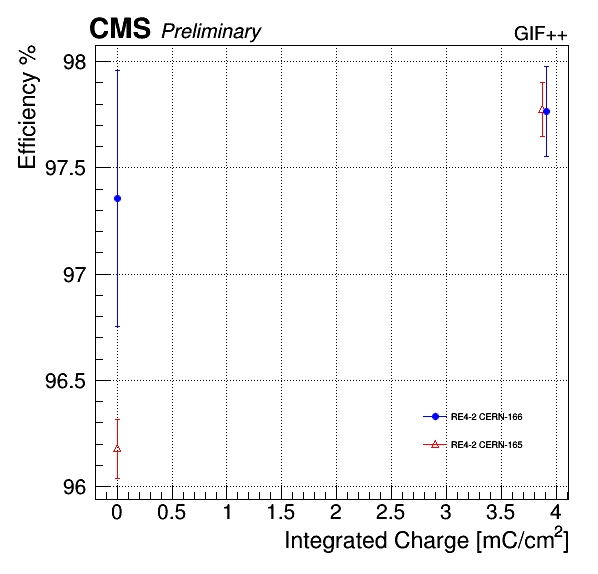
\includegraphics[width=\linewidth]{fig/chapt5/Eff-vs-Qint-RE4.png}\\
        	\caption{\label{Fig:Eff-vs-Qint:RE4}}
    	\end{subfigure}
        \caption{\label{Fig:Eff-vs-Qint} Evolution of the maximum efficiency at HL-LHC conditions, i.e. a background hit rate per unit area of \SI{300}{Hz/cm^2}, with increasing integrated charge for RE2 (\ref{Fig:Eff-vs-Qint:RE2}) and RE4 (\ref{Fig:Eff-vs-Qint:RE4}) detectors. Both irradiated (blue) and non irradiated (red) chambers are shown. The integrated charge for non irradiated detectors is recorded during test beam periods and stays small with respect to the charge accumulated in irradiated chambers.}
    \end{figure}
    
    \begin{figure}[!h]
    	\begin{subfigure}{0.5\linewidth}
			\centering
    		
\includegraphics[width=\linewidth]{fig/CMSlogo.png}\\
        	\caption{\label{Fig:Eff-Bef-Af:RE2}}
    	\end{subfigure}
    	\begin{subfigure}{0.5\linewidth}
			\centering
    		
\includegraphics[width=\linewidth]{fig/CMSlogo.png}\\
        	\caption{\label{Fig:Eff-Bef-Af:RE4}}
    	\end{subfigure}
        \caption{\label{Fig:Eff-Bef-Aft} Comparison of the efficiency sigmoid before (triangles) and after (circles) irradiation for RE2 (\ref{Fig:Eff-Bef-Af:RE2}) and RE4 (\ref{Fig:Eff-Bef-Af:RE4}) detectors. Both irradiated (blue) and non irradiated (red) chambers are shown.}
    \end{figure}
    
    \begin{figure}[!h]
    	\begin{subfigure}{0.5\linewidth}
			\centering
    		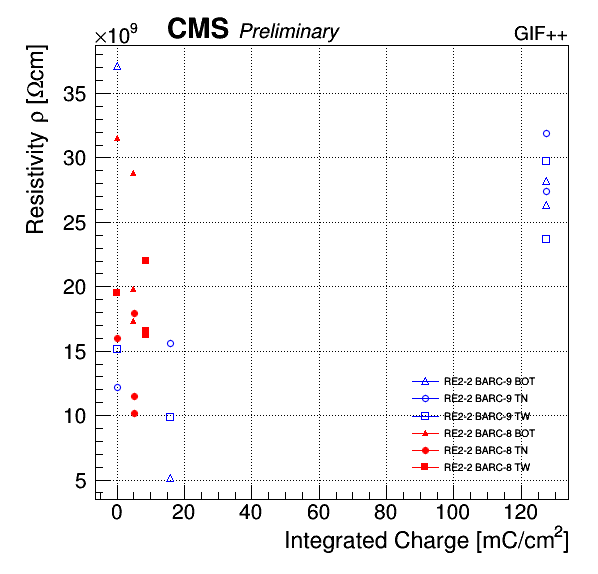
\includegraphics[width=\linewidth]{fig/chapt5/Res-vs-Qint-RE2.png}\\
        	\caption{\label{Fig:Res-vs-Qint:RE2}}
    	\end{subfigure}
    	\begin{subfigure}{0.5\linewidth}
			\centering
    		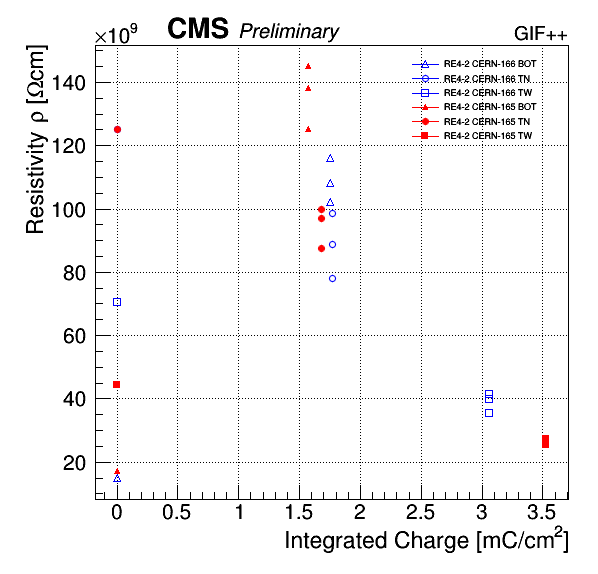
\includegraphics[width=\linewidth]{fig/chapt5/Res-vs-Qint-RE4.png}\\
        	\caption{\label{Fig:Res-vs-Qint:RE4}}
    	\end{subfigure}
        \caption{\label{Fig:Res-vs-Qint} Evolution of the Bakelite resistivity for RE2 (\ref{Fig:Res-vs-Qint:RE2}) and RE4 (\ref{Fig:Res-vs-Qint:RE4}) detectors. Both irradiated (blue) and non irradiated (red) chambers are shown.}
    \end{figure}
    
    \begin{figure}[!h]
		\centering
    	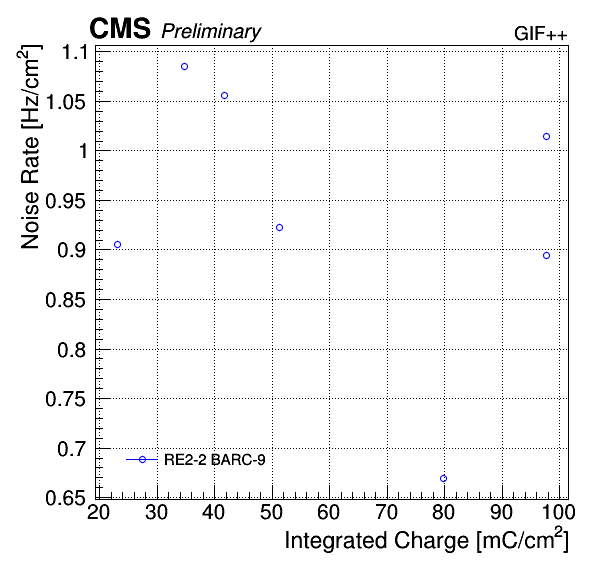
\includegraphics[width=0.5\linewidth]{fig/chapt5/Noise-vs-Qint-RE2.png}\\
        \caption{\label{Fig:Noise-vs-Qint} Evolution of the noise rate per unit area for the irradiated chamber RE2-2-BARC-9 only.}
    \end{figure}

    %******************************************** GIF++ DAQ *************************************************************************
	\subsection{Description of the \acl{DAQ}}
	\label{ssec:GIF++DAQ}

		For the longevity studies, four spare chambers of the present system are used. Two spare RPCs of the RE2,3 stations as well as two spare RPCs from the new RE4 stations have been mounted in a Trolley. Six RE4 gaps are also placed in the trolley. The trolley is placed inside the GIF++ in the upstream region of the bunker, taking the cesium source as a reference. The trolley is oriented for the detection surface of the chambers to be orthogonal to the beam line. The system can be moved along the orthogonal plane in order to have the beam in all $\eta$-partitions. For the aging the trolley is moved outside the beam line and is placed in a distance of \SI{5.2}{m} to the source, which irradiates the bunker using an attenuation filter of 2.2 which corresponds to a fluence of $10^7$\si{gamma/cm\squared}.

		During GIF++ operation, the data collected can be divided into different categories as several parameters are monitored in addition to the usual RPC performance data. On one hand, to know the performance of a chamber, it is need to measure its efficiency and to know the background conditions in which it is operated. To do this, the hit signals from the chamber are recorded and stored in a ROOT file via a \acf{DAQ} software. On the other hand, it is also very important to monitor parameters such as environmental pressure and temperature, gas temperature and humidity, RPC HV, LV, and currents, or even source and beam status. This is done through the GIF++ web \acf{DCS} that stores this information in a database.
            
		Two different types of tests are conducted on RPCs via the DAQ. Indeed, the performance of the detectors is measured periodically during dedicated test beam periods using the H4 muon beam. In between these test beam periods, when the beam is not available, the chambers are irradiated by the $^{137}$Cs in order to accumulate deposited charge and the gamma background is measured.

		RPCs under test are connected through LVDS cables to V1190A \acf{TDC} modules manufactured by CAEN. These modules, located in the rack area outside of the bunker, get the logic signals sent by the chambers and save them into their buffers. Due to the limited size of the buffers, the collected data is regularly erased and replaced. A trigger signal is needed for the TDC modules to send the useful data to the DAQ computer via a V1718 CAEN USB communication module.

		In the case of performance test, the trigger signal used for data acquisition is generated by the coincidence of three scintillators. A first one is placed upstream outside of the bunker, a second one is placed downstream outside of the bunker, while a third one is placed in front of the trolley, close by the chambers. Every time a trigger is sent to the TDCs, i.e. every time a muon is detected, knowing the time delay in between the trigger and the RPC signals, signals located in the right time window are extracted from the buffers and saved for later analysis. Signals are taken in a time window of \SI{400}{ns} centered on the muon peak (here we could show a time spectrum). On the other hand, in the case of background rate measurement, the trigger signal needs to be "random" not to measure muons but to look at gamma background. A trigger pulse is continuously generated at a rate of \SI{300}{Hz} using a dual timer. To integrate an as great as possible time, all signals contained within a time window of 10us prior to the random trigger signal are extracted form the buffers and saved for further analysis (here another time spectrum to illustrate could be useful, maybe even place both spectrum together as a single Figure).

		The signals sent to the TDCs correspond to hit collections in the RPCs. When a particle hits a RPC, it induce a signal in the pickup strips of the RPC readout. If this signal is higher than the detection threshold, a LVDS signal is sent to the TDCs. The data is then organised into 4 branches keeping track of the event number, the hit multiplicity for the whole setup, and the time and channel profile of the hits in the TDCs.

    %******************************************** GIF++ DCS *************************************************************************
	\subsection{RPC current, environmental and operation parameter monitoring}
	\label{ssec:GIF++DCS}
            
		In order to take into account the variation of pressure and temperature between different data taking periods the applied voltage is corrected following the relationship :

		\begin{equation}
			HVeff = HVapp\times\left(0.2 + 0.8\cdot\frac{P_0}{P}\times\frac{T}{T_0}\right)
		\end{equation}
		
		where $T_0$ (=\SI{293}{K}) and $P_0$ (=\SI{990}{mbar}) are the reference values.

	\subsection{Measurement procedure}
	\label{ssec:GIF++Proc}

		Insert a short description of the online tools (DAQ, DCS, DQM).\\
		Insert a short description of the offline tools : tracking and efficiency algorithm.\\
		Identify long term aging effects we are monitoring the rates per strip.
	
	%****************************************** RESULTS AT GIF++ ********************************************************************
	\subsection{Longevity studies results}
	\label{ssec:GIF++Results}

%\renewcommand*{\thesection}{\thechapter.\arabic{section}}       % reset again to chaptnum.sectnum

\clearpage{\pagestyle{empty}\cleardoublepage}
